%%%%%%%%%%%%%%%%%%%%%%%%%%%%%%%%%%%%%%%%%
% Masters/Doctoral Thesis 
% LaTeX Template
% Version 2.5 (27/8/17)
%
% This template was downloaded from:
% http://www.LaTeXTemplates.com
%
% Version 2.x major modifications by:
% Vel (vel@latextemplates.com)
%
% This template is based on a template by:
% Steve Gunn (http://users.ecs.soton.ac.uk/srg/softwaretools/document/templates/)
% Sunil Patel (http://www.sunilpatel.co.uk/thesis-template/)
%
% Template license:
% CC BY-NC-SA 3.0 (http://creativecommons.org/licenses/by-nc-sa/3.0/)
%
%%%%%%%%%%%%%%%%%%%%%%%%%%%%%%%%%%%%%%%%%

%----------------------------------------------------------------------------------------
%	PACKAGES AND OTHER DOCUMENT CONFIGURATIONS
%----------------------------------------------------------------------------------------

\documentclass[
11pt, % The default document font size, options: 10pt, 11pt, 12pt
%oneside, % Two side (alternating margins) for binding by default, uncomment to switch to one side
english, % ngerman for German
singlespacing, % Single line spacing, alternatives: onehalfspacing or doublespacing
%draft, % Uncomment to enable draft mode (no pictures, no links, overfull hboxes indicated)
%nolistspacing, % If the document is onehalfspacing or doublespacing, uncomment this to set spacing in lists to single
%liststotoc, % Uncomment to add the list of figures/tables/etc to the table of contents
%toctotoc, % Uncomment to add the main table of contents to the table of contents
%parskip, % Uncomment to add space between paragraphs
%nohyperref, % Uncomment to not load the hyperref package
headsepline, % Uncomment to get a line under the header
%chapterinoneline, % Uncomment to place the chapter title next to the number on one line
%consistentlayout, % Uncomment to change the layout of the declaration, abstract and acknowledgements pages to match the default layout
]{MastersDoctoralThesis} % The class file specifying the document structure

\usepackage[utf8]{inputenc} % Required for inputting international characters
\usepackage[T1]{fontenc} % Output font encoding for international characters

\usepackage{mathpazo} % Use the Palatino font by default

\usepackage{graphicx}
\usepackage{float}
\usepackage{minted}

\usepackage{subcaption}
\usepackage{mwe}

\usepackage[
backend=bibtex,
style=ieee,
citestyle=authoryear,
natbib=true
]{biblatex} % Use the bibtex backend with the authoryear citation style (which resembles APA)

\addbibresource{example.bib} % The filename of the bibliography

\usepackage[autostyle=true]{csquotes} % Required to generate language-dependent quotes in the bibliography

%----------------------------------------------------------------------------------------
%	MARGIN SETTINGS
%----------------------------------------------------------------------------------------

\geometry{
	paper=a4paper, % Change to letterpaper for US letter
	inner=2.5cm, % Inner margin
	outer=3.8cm, % Outer margin
	bindingoffset=.5cm, % Binding offset
	top=1.5cm, % Top margin
	bottom=1.5cm, % Bottom margin
	%showframe, % Uncomment to show how the type block is set on the page
}

%----------------------------------------------------------------------------------------
%	THESIS INFORMATION
%----------------------------------------------------------------------------------------

\thesistitle{Multi-Scale Super Resolution With Blind De-noising Using Residual Learning For Digital Art} % Your thesis title, this is used in the title and abstract, print it elsewhere with \ttitle
\supervisor{Sergio \textsc{Escalera}} % Your supervisor's name, this is used in the title page, print it elsewhere with \supname
\examiner{} % Your examiner's name, this is not currently used anywhere in the template, print it elsewhere with \examname
\degree{Master in Artificial Intelligence} % Your degree name, this is used in the title page and abstract, print it elsewhere with \degreename
\author{Santiago \textsc{Mazagatos P\'erez}} % Your name, this is used in the title page and abstract, print it elsewhere with \authorname
\addresses{} % Your address, this is not currently used anywhere in the template, print it elsewhere with \addressname

\subject{Artificial Intelligence} % Your subject area, this is not currently used anywhere in the template, print it elsewhere with \subjectname
\keywords{Super-Resolution, Residual Learning, Denoising} % Keywords for your thesis, this is not currently used anywhere in the template, print it elsewhere with \keywordnames
\university{Universitat Polit\`ecnica de Catalunya, Universitat de Barcelona, Universitat Rovira i Virgili} % Your university's name and URL, this is used in the title page and abstract, print it elsewhere with \univname
\department{} % Your department's name and URL, this is used in the title page and abstract, print it elsewhere with \deptname
\group{} % Your research group's name and URL, this is used in the title page, print it elsewhere with \groupname
\faculty{} % Your faculty's name and URL, this is used in the title page and abstract, print it elsewhere with \facname

\AtBeginDocument{
\hypersetup{pdftitle=\ttitle} % Set the PDF's title to your title
\hypersetup{pdfauthor=\authorname} % Set the PDF's author to your name
\hypersetup{pdfkeywords=\keywordnames} % Set the PDF's keywords to your keywords
}

\begin{document}

\frontmatter % Use roman page numbering style (i, ii, iii, iv...) for the pre-content pages

\pagestyle{plain} % Default to the plain heading style until the thesis style is called for the body content

%----------------------------------------------------------------------------------------
%	TITLE PAGE
%----------------------------------------------------------------------------------------

\begin{titlepage}
\begin{center}

\vspace*{.06\textheight}
\textsc{\Large Universitat Polit\`ecnica de Catalunya - Facultat d'Inform\`atica de Barcelona}\\[0.5cm]
\textsc{\Large Universitat de Barcelona - Facultat de Matem\`atiques}\\[0.5cm]
\textsc{\Large Universitat Rovira i Virgili - Escola T\`ecnica Superior d'Enginyeria}\\[1cm]
\textsc{\Large Master Thesis}\\[0.5cm] % Thesis type

\HRule \\[0.4cm] % Horizontal line
{\huge \bfseries \ttitle\par}\vspace{0.4cm} % Thesis title
\HRule \\[1.5cm] % Horizontal line
 
\begin{minipage}[t]{0.4\textwidth}
\begin{flushleft} \large
\emph{Author:}\\
{\authorname} % Author name - remove the \href bracket to remove the link
\end{flushleft}

\end{minipage}
\begin{minipage}[t]{0.4\textwidth}
\begin{flushright} \large
\emph{Advisor:} \\
{\supname} % Supervisor name - remove the \href bracket to remove the link  
\end{flushright}
\end{minipage}\\[3cm]
 
\vfill

{\large April 24, 2019}\\[4cm] % Date
%\includegraphics{Logo} % University/department logo - uncomment to place it
 
\vfill
\end{center}
\end{titlepage}

%----------------------------------------------------------------------------------------
%	ABSTRACT PAGE
%----------------------------------------------------------------------------------------

\begin{abstract}
\addchaptertocentry{\abstractname} % Add the abstract to the table of contents
 In the fields of illustration and digital art, it is imperative that an image be of high quality when being used for printing, as a wallpaper or for another kind of decorative purpose, however, high resolution, clean images are often unavailable, either because the form in which the original work was rendered is deemed subpar by today’s standards, or because all available copies have been subject to lossy compression or downsampling. Super Resolution is an increasingly active field of research in machine learning with the aim of providing a computational model that can achieve what is impractical or impossible with human means, the recreation of available images or other kind of visual data in the highest possible quality, in my work I make use of state-of-the-art Super-Resolution methods and denoising methods to try and create a comprehensive solution for all use cases related to digital art restoration.
\end{abstract}
\keywordnames

%----------------------------------------------------------------------------------------
%	LIST OF CONTENTS/FIGURES/TABLES PAGES
%----------------------------------------------------------------------------------------

\tableofcontents % Prints the main table of contents

\listoffigures % Prints the list of figures

%\listoftables % Prints the list of tables

%----------------------------------------------------------------------------------------
%	THESIS CONTENT - CHAPTERS
%----------------------------------------------------------------------------------------

\mainmatter % Begin numeric (1,2,3...) page numbering

\pagestyle{thesis} % Return the page headers back to the "thesis" style

% Include the chapters of the thesis as separate files from the Chapters folder
% Uncomment the lines as you write the chapters

% Chapter Template

\chapter{Introduction} % Main chapter title

\label{Chapter1} % Change X to a consecutive number; for referencing this chapter elsewhere, use \ref{ChapterX}

Technical limitations are as common to technology as technology itself, what was a vast amount of storage a decade ago is little more than what one would expect from a basic cloud storage plan today, that being the case one often comes face to face with yesterday's limitations, chief among them processing power and storage.

\hfill

In an era in which the most common removable storage medium had no more than 1.44 Megabytes of space and the average processor had its performance measured in Megahertz and whether or not it had a math co-processor, image use was accompanied by lossy compression, like in the case of JPEG (\cite{JPEG}) files, to save the most amount of space, and cheap downsampling methods that wouldn't overburden the CPU.

\hfill

Nowadays storing images in PNG (\cite{PNG}) format with its lossless compression and downsizing using methods such as Lanczos resampling (\cite{wiki:Lanczos}) to prevent aliasing is a reasonable proposition, but the previous methods of saving space and cycles are still present, and there's no way of knowing whether an illustration created by a digital artist today with a high definition display will end up being dwarfed by screens 10 years into the future.

\hfill

If one wanted to print an illustration onto a T-shirt, or a poster, or use it as a wallpaper on a 4K display, such file would need to have a very high resolution and no compression artifacts or noise to look good, however such files can often only be sourced from the artist, if they even exist; recreating the work in a way that achieves the required quality would require a substantial amount of time and effort by someone with the skill set to do so, while it would be expensive for someone who lacks it to commission someone for it, furthermore the result might still be unsatisfactory, with the recreated image having a slightly different aesthetic feel to it.

\section{Waifu2x}

Waifu2x (\cite{waifu2x}) is a web based application that performs upscaling and denoising of anime style images and photos, however, it uses different models for different levels of noise, relying on the user to select the correct denoising level, and it only allows upscaling up to 2 times the original image size.

\hfill

While there is a Caffe port of waifu2x (\cite{waifu2x-caffe}) that supports upscaling beyond 2 times and has an auto-denoising feature, it is not explained how the software determines the best denoising level for a particular image, this port runs on the user's computer and is able to take advantage of any CUDA enabled graphics cards present, making it well suited for batch processing images since the original web application has no such feature and requires a captcha to be resolved for every processed image.

\section{Goals}

The goals of this project are simple, to create a model that is able of upscaling and denoising an image (digital art) without any prior knowledge of level or type of noise (if any) present on the input image/s with results on par or superior to those of the best available alternative (Waifu2x).


\chapter{State of the art} % Main chapter title

\label{Chapter2}

\section{Super-Resolution}

Initial works in the world of Super-Resolution relied primarily on Dictionary based approaches, with low resolution and high resolution dictionaries in which a high resolution image is obtained by matching the low resolution representation to items in the LR dictionary and translating those similarities using the HR dictionary to the final HR image.

\hfill 

Dictionary based methods have undergone a great deal of transformation, with a wide array of improvements designed to improve the dictionary learning process (\cite{BPJDL}), or the LR to HR mapping in terms of speed and memory with approaches like Anchor Neighborhood Regression (\cite{ANR}), with its subsequent improvements(\cite{APlus}, \cite{IA}, \cite{PSyCo}), Sparse Coding (\cite{SC}, \cite{CSCN}) and Super-Resolution Forests (\cite{NBSRF}, \cite{RFL}).

\hfill

Along with all the methods reliant on external information came the ones reliant in information intrinsic to the images being processed (\cite{SelfEx}) and more hybrid approaches with external pre-training and internal fine tuning (\cite{DJSR}.

\hfill

However, present works rely on less engineered solutions with maps of LR and HR dictionaries and instead have networks learn the mapping functions directly in a non-linear way, the specifics still vary depending on which mapping function has to be learned, the primary example of this new avenue of research is SRCNN (\cite{SRCNN}), which has been the subject of some improvements (\cite{ESPCN}, \cite{FSRCNN}).

\hfill

As models were made deeper in order to learn more complex mappings, skip connections like the ones displayed in ResNet (\cite{ResNet}) were added to avoid exploding/vanishing gradients (\cite{DRRN}, \cite{VDSR}, \cite{SRGAN}, \cite{EDSR}), recursive architectures have also been successfully implemented, among other things as a way to mitigate overfitting (\cite{DRCN}), which have then been improved upon (\cite{DRRN}) 

\hfill

Additionally, new models have been using Generative Adversarial Networks as a way of guiding networks towards producing results belonging to the natural image manifold, avoiding results that are good number-wise (as in having a low Mean Squared Error, or high PSNR and SSIM), but look "soft" and artificial to humans. (\cite{SRGAN}, \cite{SFT-GAN}, \cite{CinCGAN}).

\subsection{Denoising}

Modern denoising methods often double as SISR models, such as TNRD (\cite{TNRD}) and RED30 (\cite{RED30}), and despite its age, BM3D (\cite{BM3D}) is still relevant and being revisited, either to propose an alternative (\cite{MLP-BM3D}), or a modern adaptation (\cite{BM3D-Net}). 

\section{Deep Learning libraries}

There are a variety of Open Source machine learning libraries for Python with CUDA support:

\begin{itemize}
    \item \textbf{TensorFlow}: Developed by the Google Brain Team, TensorFlow is a very popular library, especially when used as a backend with Keras, it is in fact taught in this Master's Deep Learning course. (\cite{tensorflow})
    \item \textbf{PyTorch}: Based on Torch and merged with Caffe2, it is developed by Facebook's AI research group. (\cite{pytorch})
    \item \textbf{Theano}: While no longer in development and a relatively minor player, the fact that it was developed by the Montreal Institute for Learning Algorithms might attract those who might be displeased with the corporate ties of other libraries. (\cite{theano})
    \item \textbf{Microsoft Cognitive Toolkit}: Microsoft's CNTK library has both a Python API and a C\# API, which makes it much easier to integrate with Universal Windows Platform, Windows Forms and ASP.NET applications. (\cite{cntk})
\end{itemize}
\chapter{Methodology} % Main chapter title

\label{Chapter3}

\section{Choice: EDSR vs. CinCGAN}

At the start of this master thesis project my advisor gave me two papers as good state of the art methods that would do nicely EDSR (\cite{EDSR}) and CinCGAN (\cite{CinCGAN}) offer fundamentally different approaches to Super Resolution:

\hfill

EDSR builds on SRResNet (\cite{SRGAN}), which is an adaptation of ResNet (\cite{ResNet}) for SISR, removing Batch Normalization layers, thus reducing the computational and memory burden of the network on hardware and allowing for a deeper architecture and more complex non-linear model to be learned for LR/HR mapping. 

\hfill

CinCGAN uses CycleGAN's (\cite{CycleGAN}) idea of image to image translation to create an unsupervised model that can denoise and upsample images without training with LR/HR pairs by first denoising the input in LR space, and then upscaling it with a state of the art SISR model, in this case EDSR.

\hfill

While CinCGAN achieves performance comparable to SRGAN, I personally find CinCGAN's results visually un-appealing since it seems to introduce artifacts of its own.

\hfill

\begin{figure}[H]
\centering
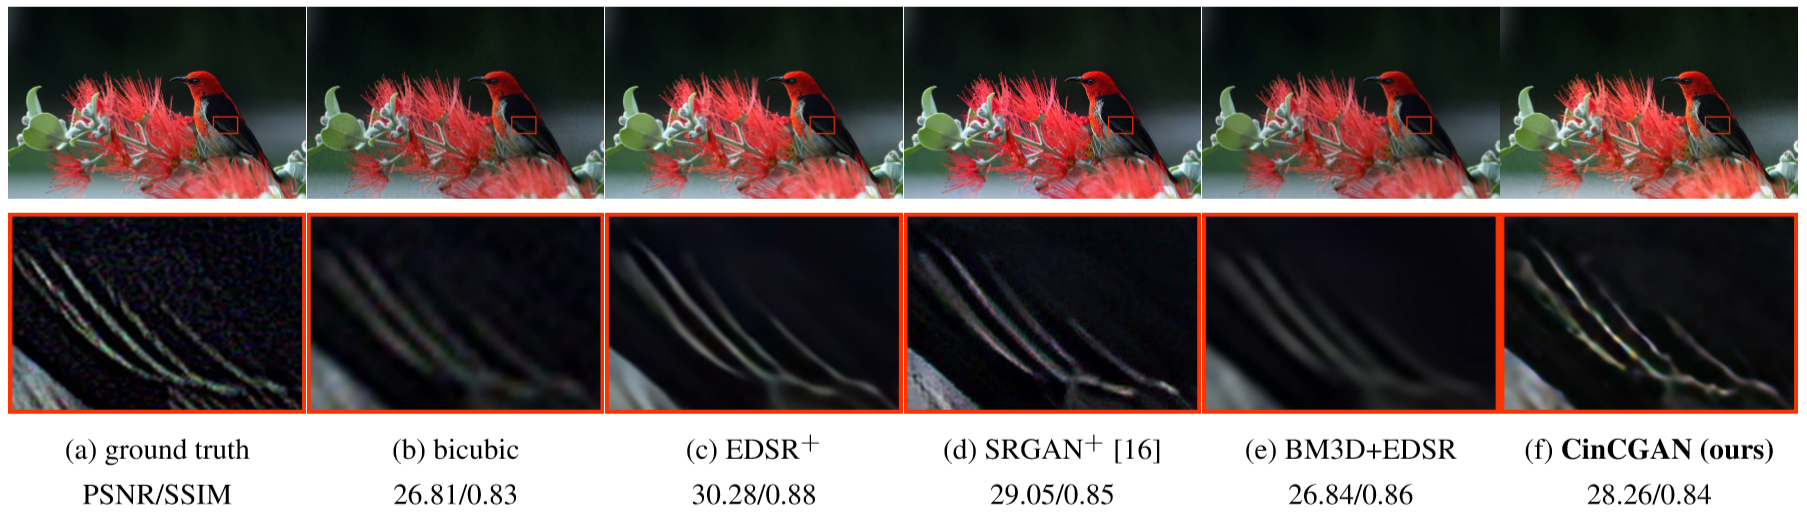
\includegraphics[width=\textwidth]{../Figures/CinCGAN2}
\caption{While SRGAN+'s result is not as sharp as the ground truth or CinCGAN's result, the lines in the latter case look distorted (Taken from the CinCGAN paper)}
\end{figure}

\begin{figure}[H]
\centering
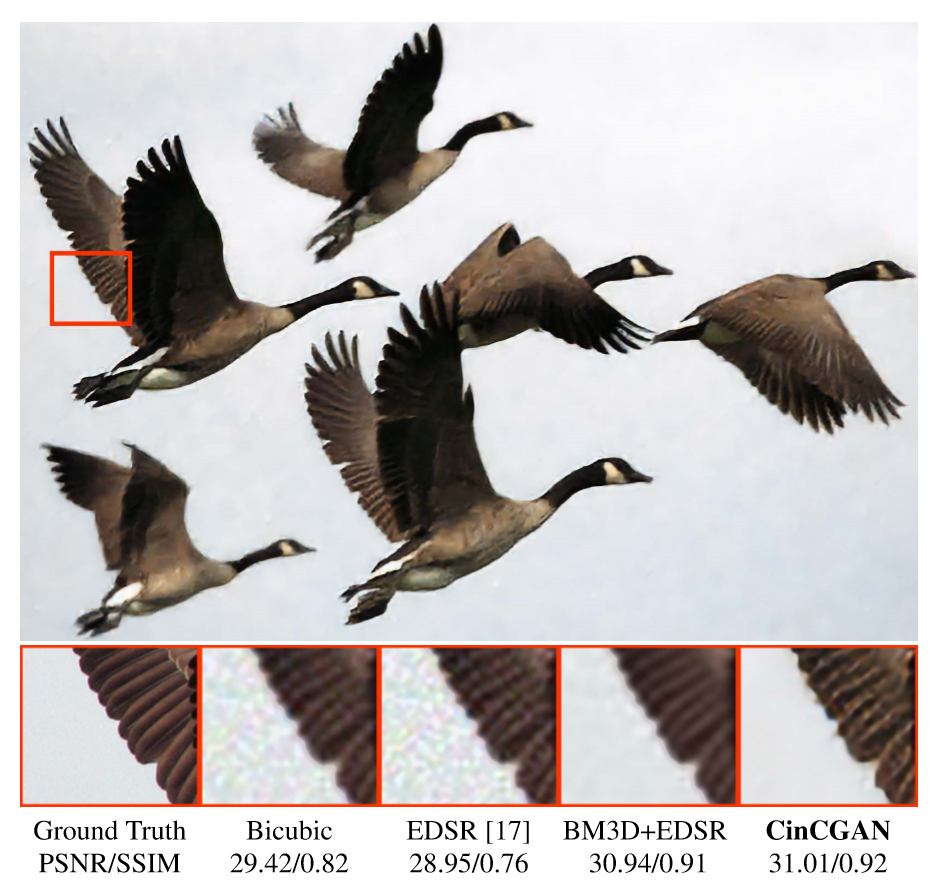
\includegraphics[width=0.75\textwidth]{../Figures/CinCGAN1}
\caption{While Bicubic and EDSR models can't denoise the image and BM3D+EDSR's result looks soft and blurry, the CinCGAN seems to introduce its own noise (Taken from the CinCGAN paper)}
\end{figure}

Since EDSR already performed the SR task inside CinCGAN and I didn't like the visual quality of the results given by the latter I chose to work with EDSR as a SR method, and would later think of a way of performing denoising.

\section{Choice: Denoising}

Denoising is a much more established and "stable" field, so when faced with the need to choose a denoising method I chose to look for extensively cited papers first instead of prioritizing state-of-the-art brand new ones.

\hfill

DnCNN (\cite{DnCNN}) is a residual neural network capable of handling gaussian noise and JPEG compression, its architecture according to the authors is a modified VGG (\cite{VGG}) network, adapting it for denoising instead of image recognition and implementing residual learning (\cite{ResNet}), the result is strikingly similar to SRResNet, and therefore, to EDSR, although SR tasks in DnCNN are performed by upscaling a LR image to HR size using bicubic interpolation and feeding it to the network.

\hfill

The way training data is created for DnCNN is to create patches with noise in the ranges of [0,55]$\sigma$ for gaussian noise and [5,99] quality for JPEG deblocking.

\hfill

I hypothesized that I could take the training method in DnCNN and use it with the EDSR architecture, since the only major differences were the lack of Batch Normalization layers, and the deconvolution and transpose process at the very end of EDSR, making its output larger than its input.

\hfill

DnCNN had been tested without Batch Normalization and it was shown that with Adam (\cite{Adam}), the training and performance impact of not using BN layers was small, so that wouldn't be a significant issue.

\begin{figure}[H]
\centering
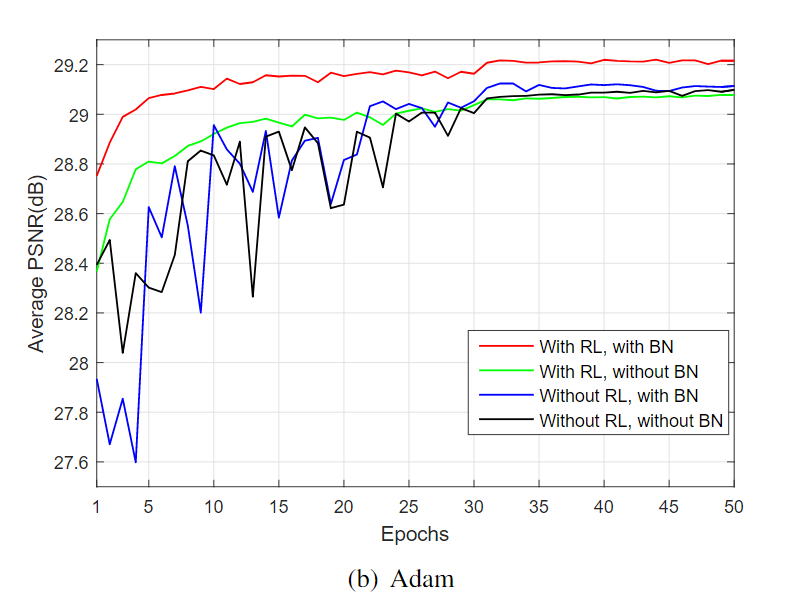
\includegraphics[width=0.75\textwidth]{../Figures/DnCNNAdam}
\caption{Impact of training DnCNN with and without BN (Taken from the DnCNN paper)}
\end{figure}

\section{Final decision}

I chose to use the EDSR architecture with a mixed training approach, the images in the training set would be split into overlapping patches, augmented with 90 degree rotations and then treated randomly in one of three ways (in all cases the HR patch is saved as a PNG intact):

\hfill

\begin{itemize}
    \item \textbf{Clean save}: the extracted patch would be downscaled using Lanczos resampling and saved as a PNG to preserve its quality.
    \item \textbf{JPEG save}: the extracted patch would be downscaled using Lanczos resampling and saved as a JPEG with a quality varying from 5 to 99.
    \item \textbf{Gauss save}: the extracted patch would be downscaled using Lanczos resampling, gaussian noise would be added to the patch with a standard deviation value between 0 and 55 and then saved as a PNG file.
\end{itemize}

\hfill

The network will follow the EDSR architecture and be trained with the Adam optimizer (learning rate: 1e-4, with it being halved every 200.000 updates, momentum: 0.9, variance momentum: 0.999, $\epsilon$: 1e-8) for 300.000 updates with a minibatch size of 16, for the loss function, L2 is used (as in SRResNet) instead of L1 (EDSR).

\begin{figure}[H]
\centering
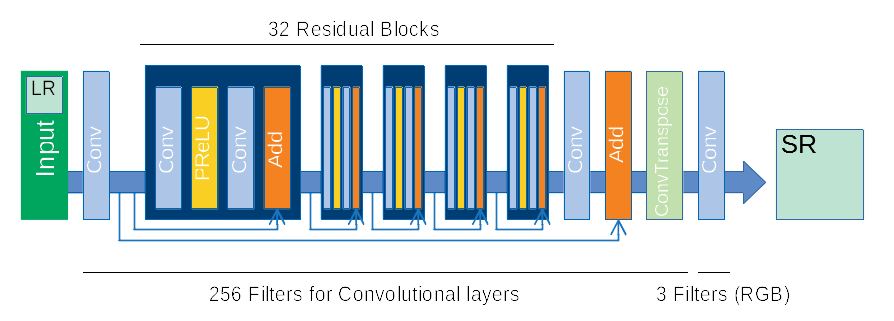
\includegraphics[width=0.75\textwidth]{../Figures/EDSR_Arch}
\caption{Implemented Architecture for 2x and 3x scales}
\end{figure}

\hfill

This for 4X upscaling has one more ConvolutionTranpose layer, this is especially useful for reusing the 2X model's weights to train a 4X model since the parameters of the layer remain the same.

\chapter{Development} % Main chapter title

\label{Chapter4}

\section{Dataset}

To train the model to work with digital art and illustrations a dataset other than the usual photograph based datasets like the ones used on the EDSR paper (DIV2K, Set5, Set14, B100, Urban100), to do that I considered a variety of digital art imageboards: Danbooru, Gelbooru, Yandere, e621, Sankaku Channel and Derpibooru.

\hfill

I needed images that were in PNG format, for practicality reasons the selected board had to work well with an automatic downloader (\cite{grabber}), the board from which the images were going to be downloaded also needed to have reliable tagging and preferably, an active community that would use the often underutilized scoring system present in (nearly) all imageboards.

\hfill

Danbooru and e621 were the best candidates among all imageboards considered but due to the prevalence of japanese artists in Danbooru and their infamous censorship practices I chose e621 over Danbooru to ensure no mosaic filters ended up in the training patches.

\hfill

I downloaded the 1,600 highest scored images on e621 with the assumption that due to their popularity they would be more representative of what the final use case would be.

\section{Network implementation}

Microsoft's CNTK has a greater amount of instructional materials, including examples and tutorials than TensorFlow (in my experience), and has a guide on how to implement various SISR models such as VDSR, DRRN, SRResNet and SRGAN and how to use them later to upscale images (\cite{cntk-tutorial})

\hfill

The reason why 1,600 images were downloaded (an excessive amount) is because I initially considered adding a discriminator to EDSR, effectively applying EDSR's improvements over SRResNet to SRGAN and I would use 800 images to train the generator, and 800 to train the GAN, however SRGAN relies on a pre-trained VGG network which is trained on different data (photographs) and training the discriminator from scratch, fine tuning the balance in the loss function between discriminator and generator was a dangerous timesink.

\hfill

Due to memory constraints on my GTX 1060 (6 GB), the LR patch size for the network had to be reduced to 32 x 32, down from EDSR's LR patch size of 48 x 48.

\begin{figure}[H]
\centering
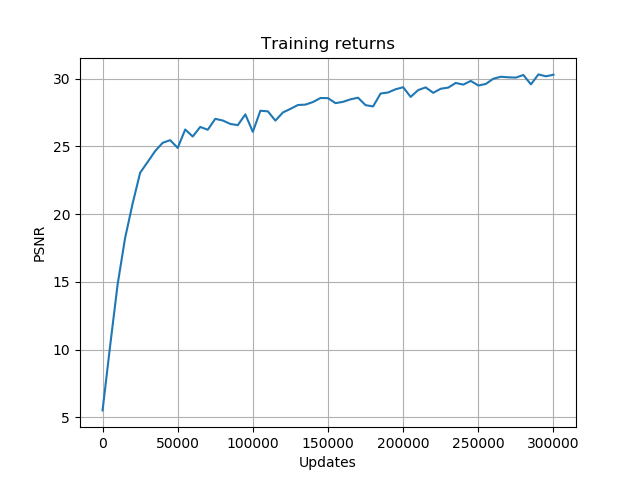
\includegraphics[width=0.75\textwidth]{../Figures/PSNR_Training_Curve}
\caption{Training curve for 2X scale, Training time was: 1 day, 22 hours, 53 minutes}
\end{figure}

\hfill

Geometric Self Ensemble as used in \cite{EDSR} and explained in \cite{IA} was implemented, however I haven't used it for testing purposes, my concerns being that each patch needs to be predicted 8 times and the same concerned expressed by \cite{SRGAN} in section 1.1.3, being that averaging all possible solutions for a specific patch might cause a loss of detail and overly smooth the image as a whole, since EDSR doesn't have a discriminator to ensure a good perceptual loss value, this issue is especially relevant.

\section{Graphical User Interface}

Using waifu2x-caffe as an inspiration I created a graphical user interface designed not only to use my EDSR models, but any CNTK model that takes low resolution patches and outputs high resolution ones, the code only needs to know the output patch size and the upscaling coefficient and it will deconstruct input images into appropriately sized patches and reconstruct a high resolution image from the results, additionally, unlike waifu2x-caffe, this GUI presents a real time preview of the upscaling process, a lack of feedback can often be upsetting to users especially if the model is being run on slow hardware.

\hfill

\begin{figure}[H]
\centering
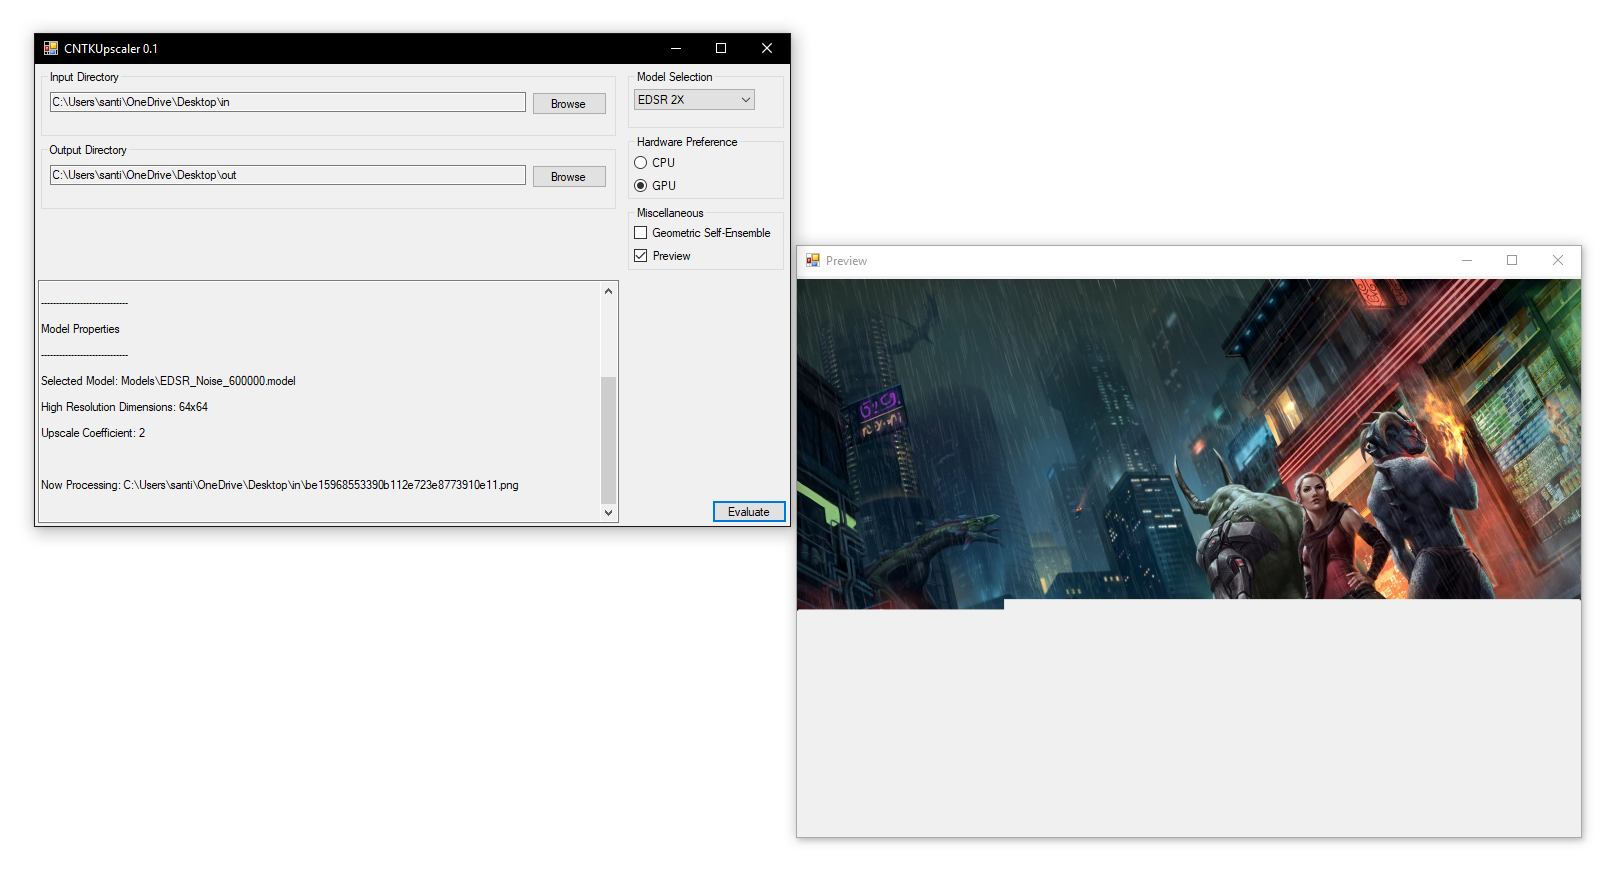
\includegraphics[width=\textwidth]{../Figures/CNTKUpscaler_screenshot}
\caption{Screenshot of the CNTK Upscaler GUI}
\end{figure}

\hfill

The upscaler also supports using Geometric Self Ensemble since it isn't dependent on the model, and models can be added by placing them on the 'Models' folder of the application along with a JSON file with the necessary information, the application automatically loads all models present in the folder at startup.

\hfill

\begin{figure}[H]
\centering
\begin{minted}{json}
{
  "ModelName": "EDSR 2X",
  "File": "EDSR_Noise_600000.model",
  "OutDimensions": 64,
  "UpscaleCoefficient": 2
}
\end{minted}
\caption{An example JSON file}
\end{figure}
\chapter{Evaluation} % Main chapter title

\label{Chapter5}

To evaluate the trained EDSR with blind-denoising I hand picked 7 pictures with varying styles and complexity and created low resolution versions with specific gaussian noise levels and JPEG qualities; for Gaussian noise the $\sigma$ values were: 0, 15, 25 and 50. And for JPEG quality levels, the values were: 25, 50, 75 and 100, in total that is 56 low resolution images per model to test.

\hfill

\begin{figure}[H]
        \centering
        \begin{subfigure}[b]{0.475\textwidth}
            \centering
            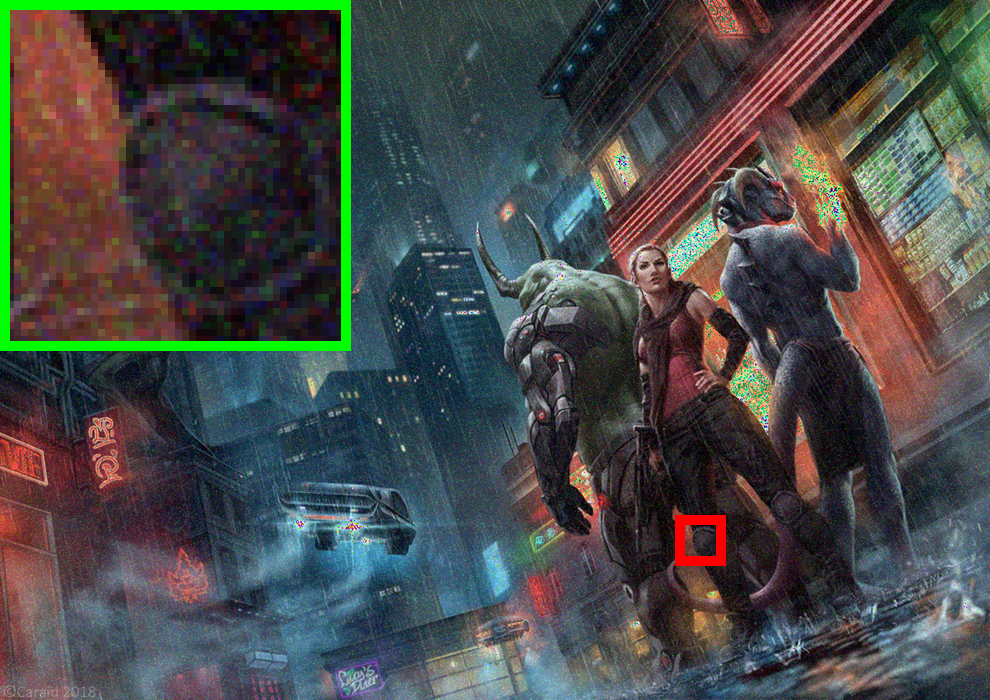
\includegraphics[width=\textwidth]{Figures/2X/Cyberpunk/LR_Cyberpunk_GAUSS_25_comparison.png}
            \caption{LR image with gaussian noise (25$\sigma$)}
        \end{subfigure}
        \hfill
        \begin{subfigure}[b]{0.475\textwidth}  
            \centering 
            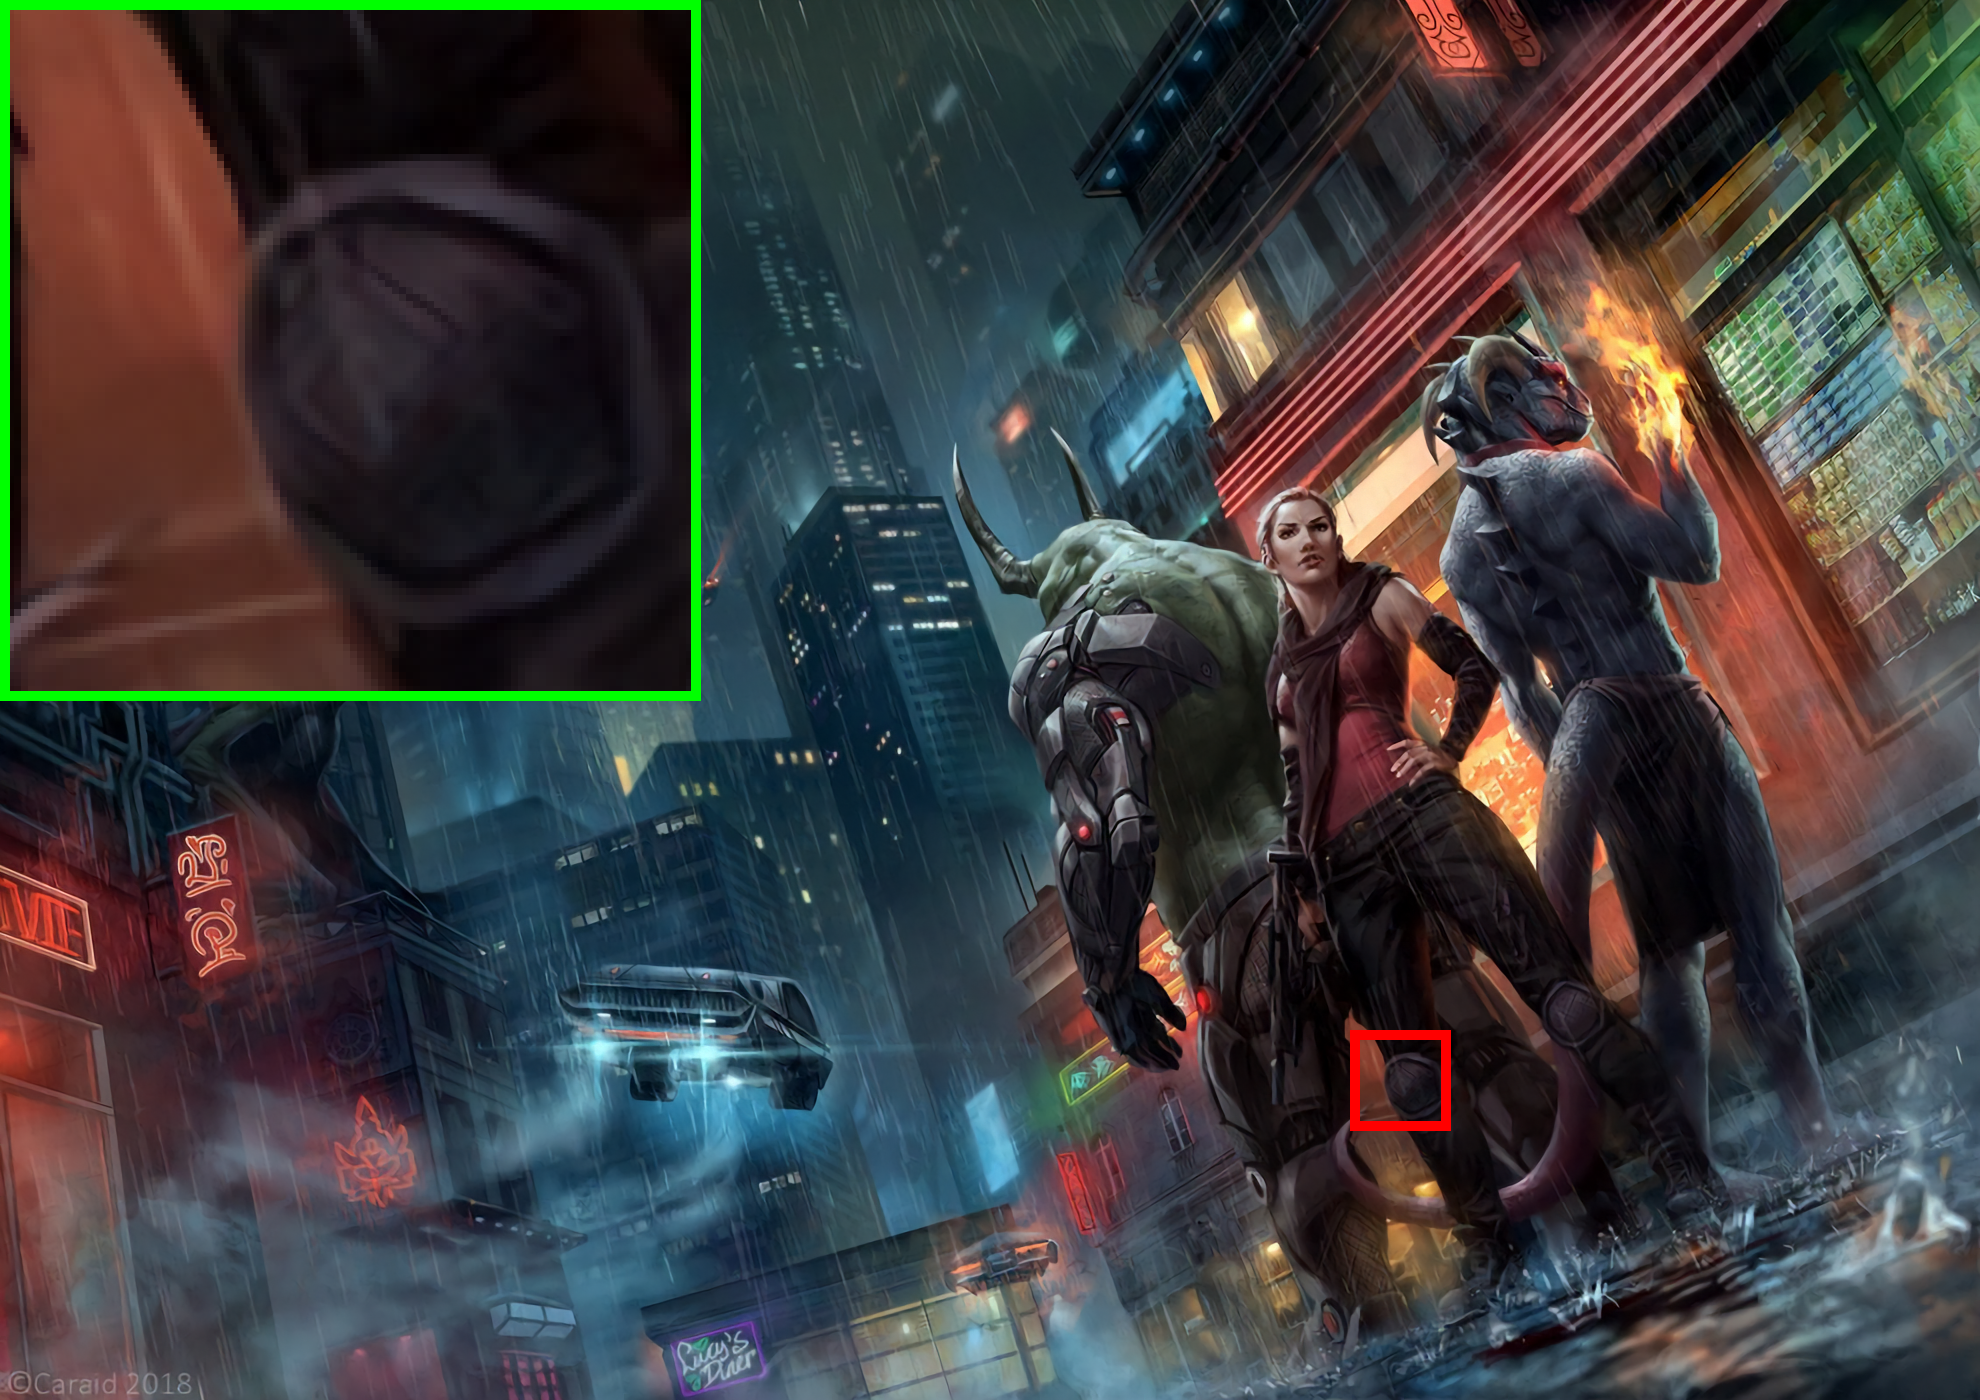
\includegraphics[width=\textwidth]{Figures/2X/Cyberpunk/EDSR_Cyberpunk_GAUSS_25_comparison.png}
            \caption{EDSR result}
        \end{subfigure}
        \vskip\baselineskip
        \begin{subfigure}[b]{0.475\textwidth}   
            \centering 
            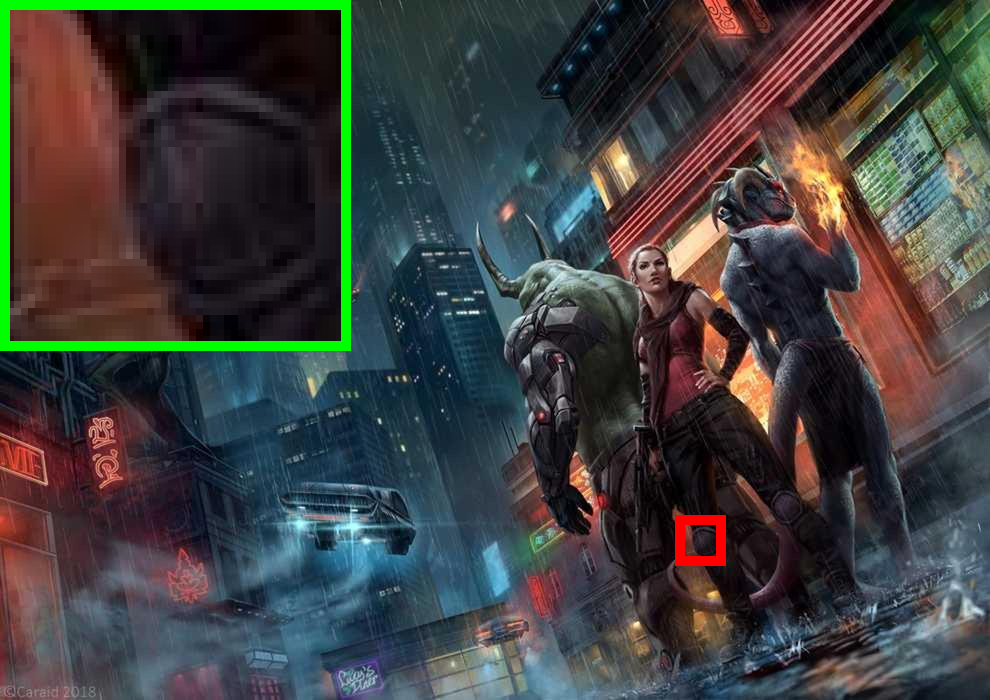
\includegraphics[width=\textwidth]{Figures/2X/Cyberpunk/LR_Cyberpunk_JPEG_50_comparison.png}
            \caption{LR image with JPEG noise (50)}
        \end{subfigure}
        \quad
        \begin{subfigure}[b]{0.475\textwidth}   
            \centering 
            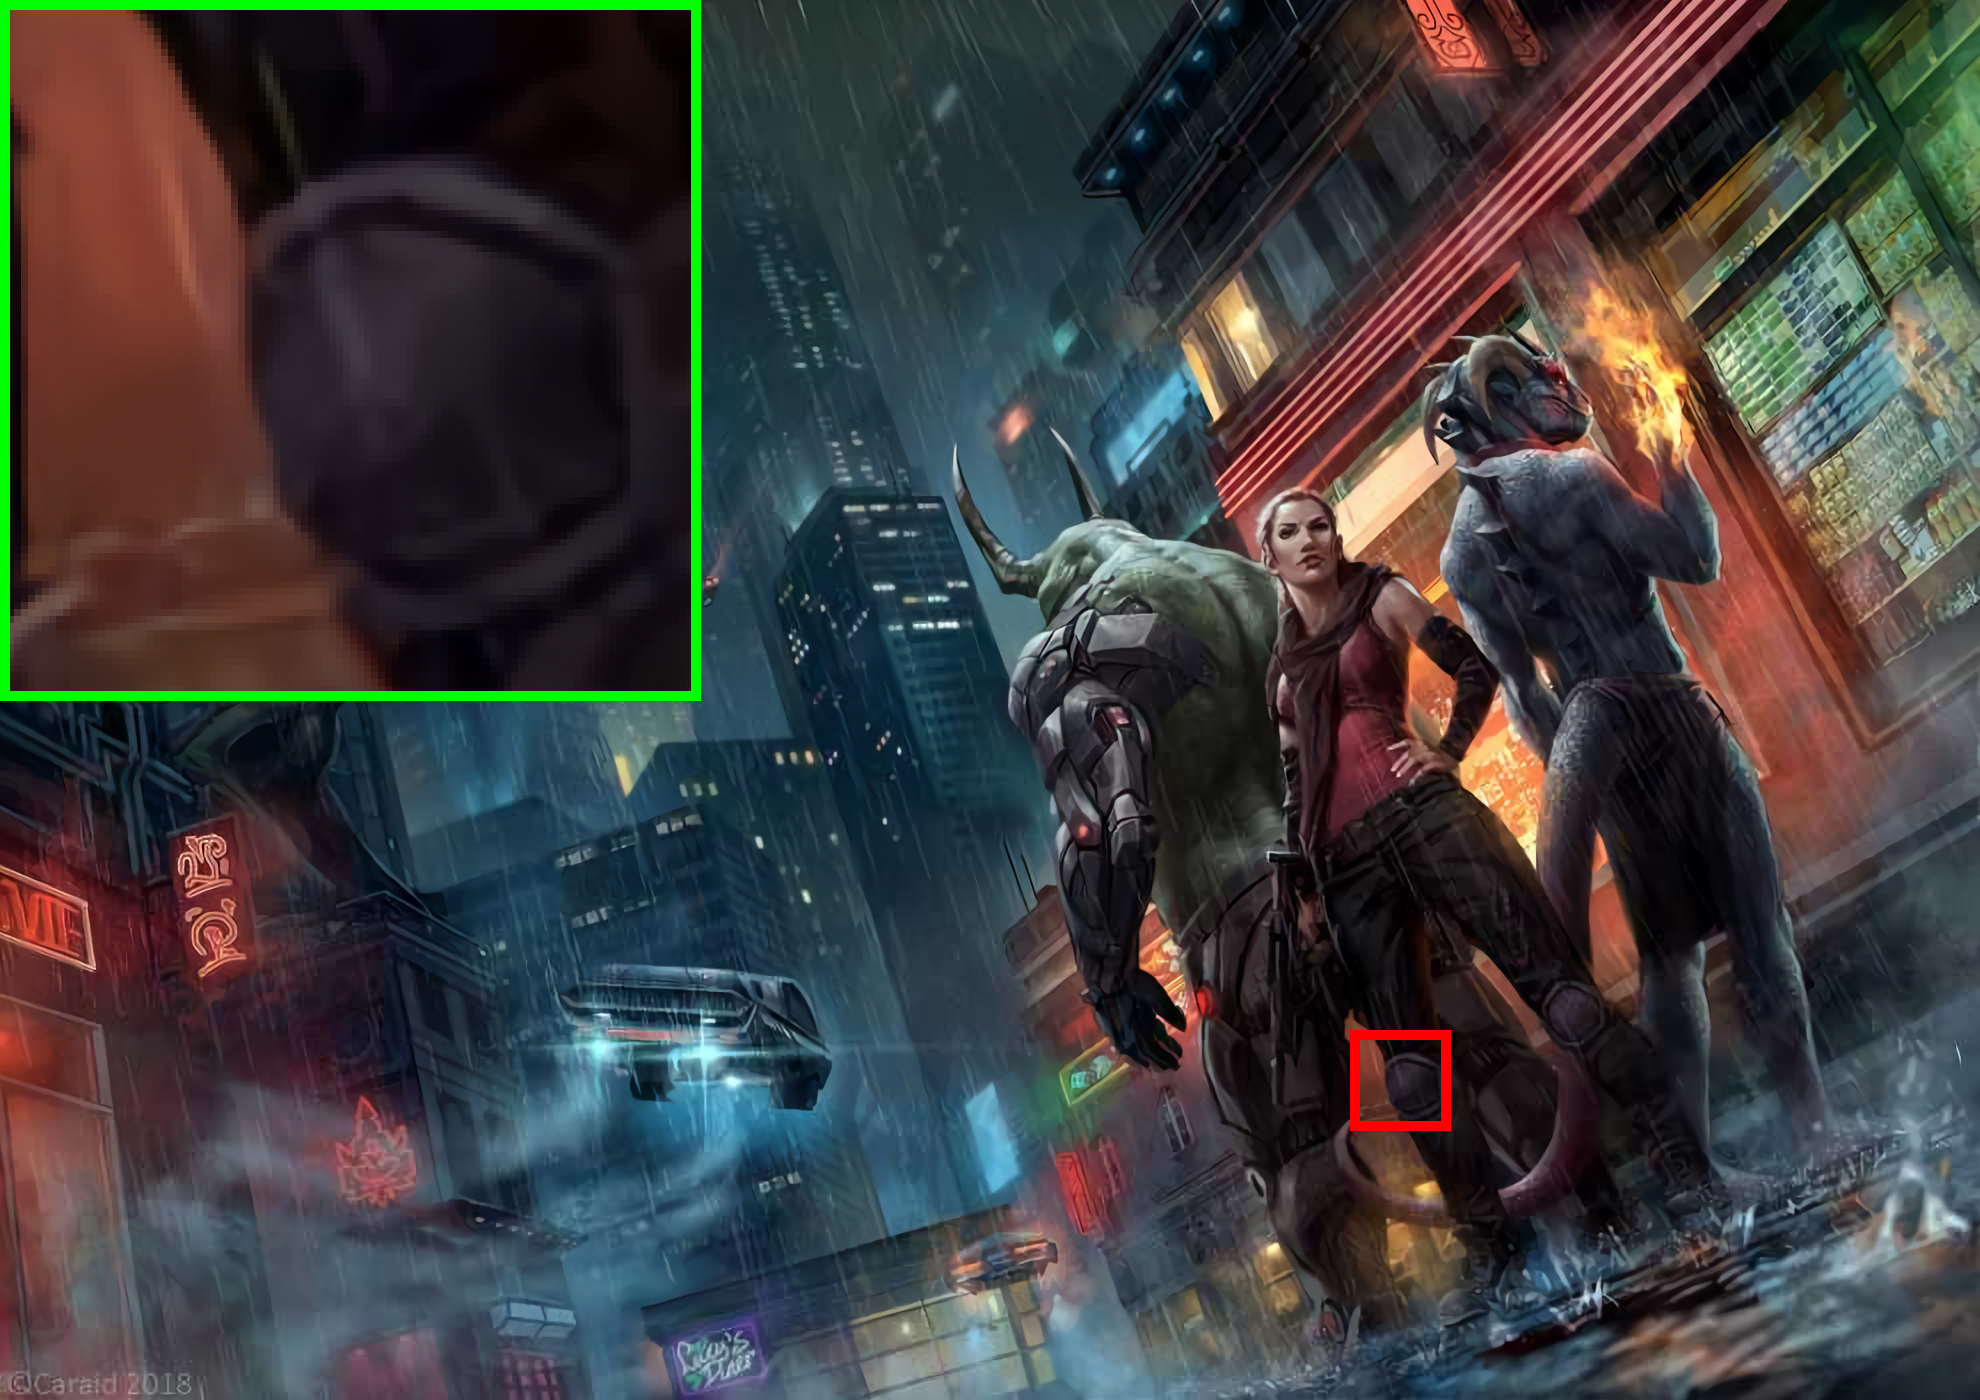
\includegraphics[width=\textwidth]{Figures/2X/Cyberpunk/EDSR_Cyberpunk_JPEG_50_comparison.png}
            \caption{EDSR result}
        \end{subfigure}
        \caption{trained denoising capabilities}
\end{figure}


\begin{figure*}
        \centering
        \begin{subfigure}[b]{0.475\textwidth}
            \centering
            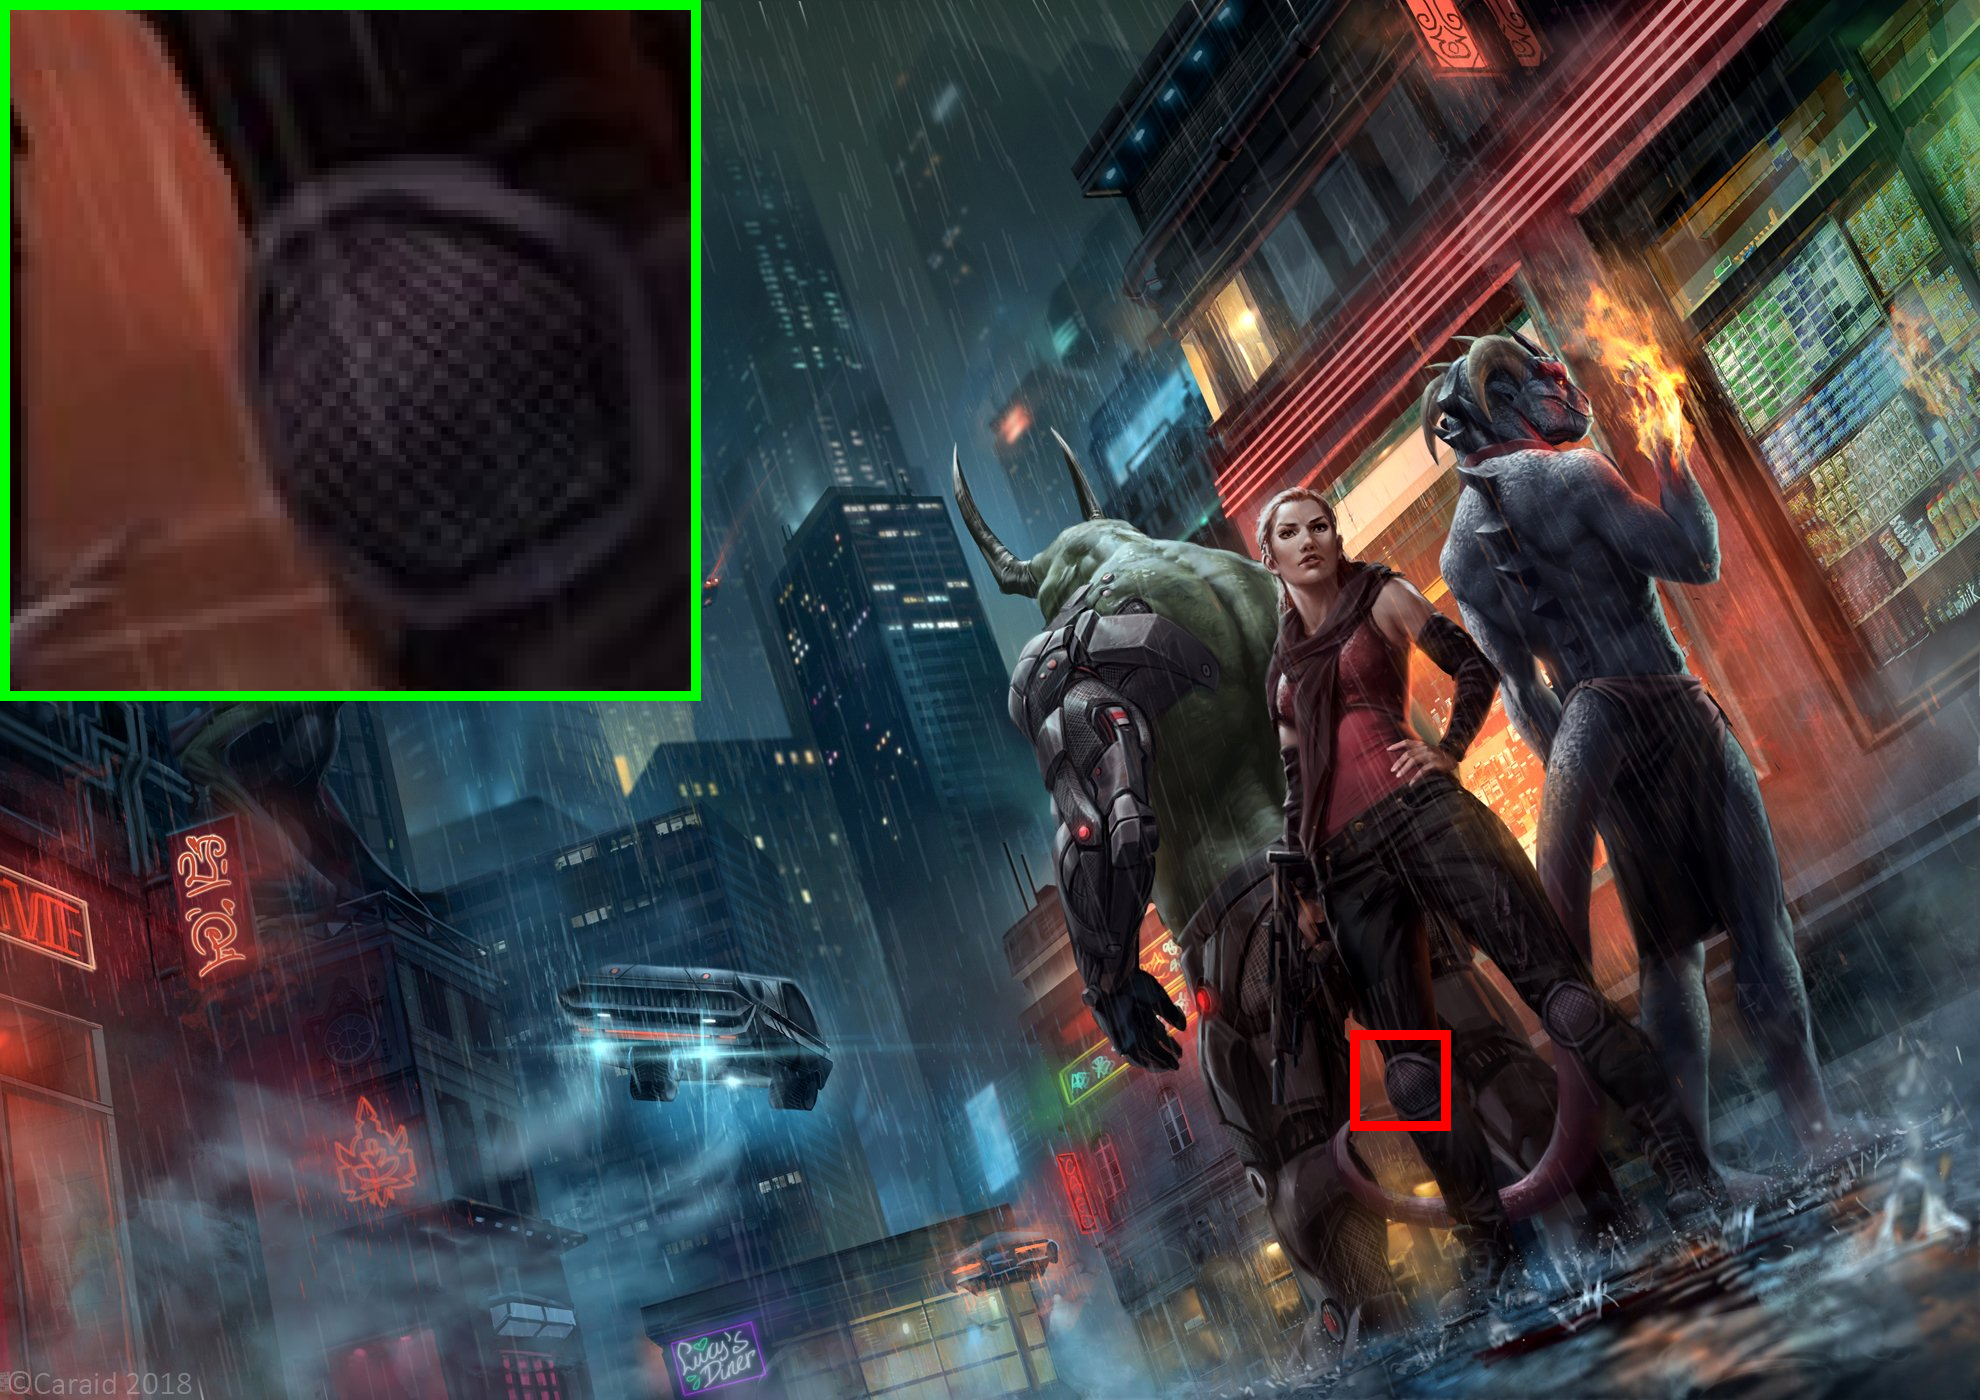
\includegraphics[width=\textwidth]{Figures/2X/Cyberpunk/Cyberpunk_HR.png}
            \caption{High Resolution}
        \end{subfigure}
        \vskip\baselineskip
        \begin{subfigure}[b]{0.475\textwidth}
            \centering
            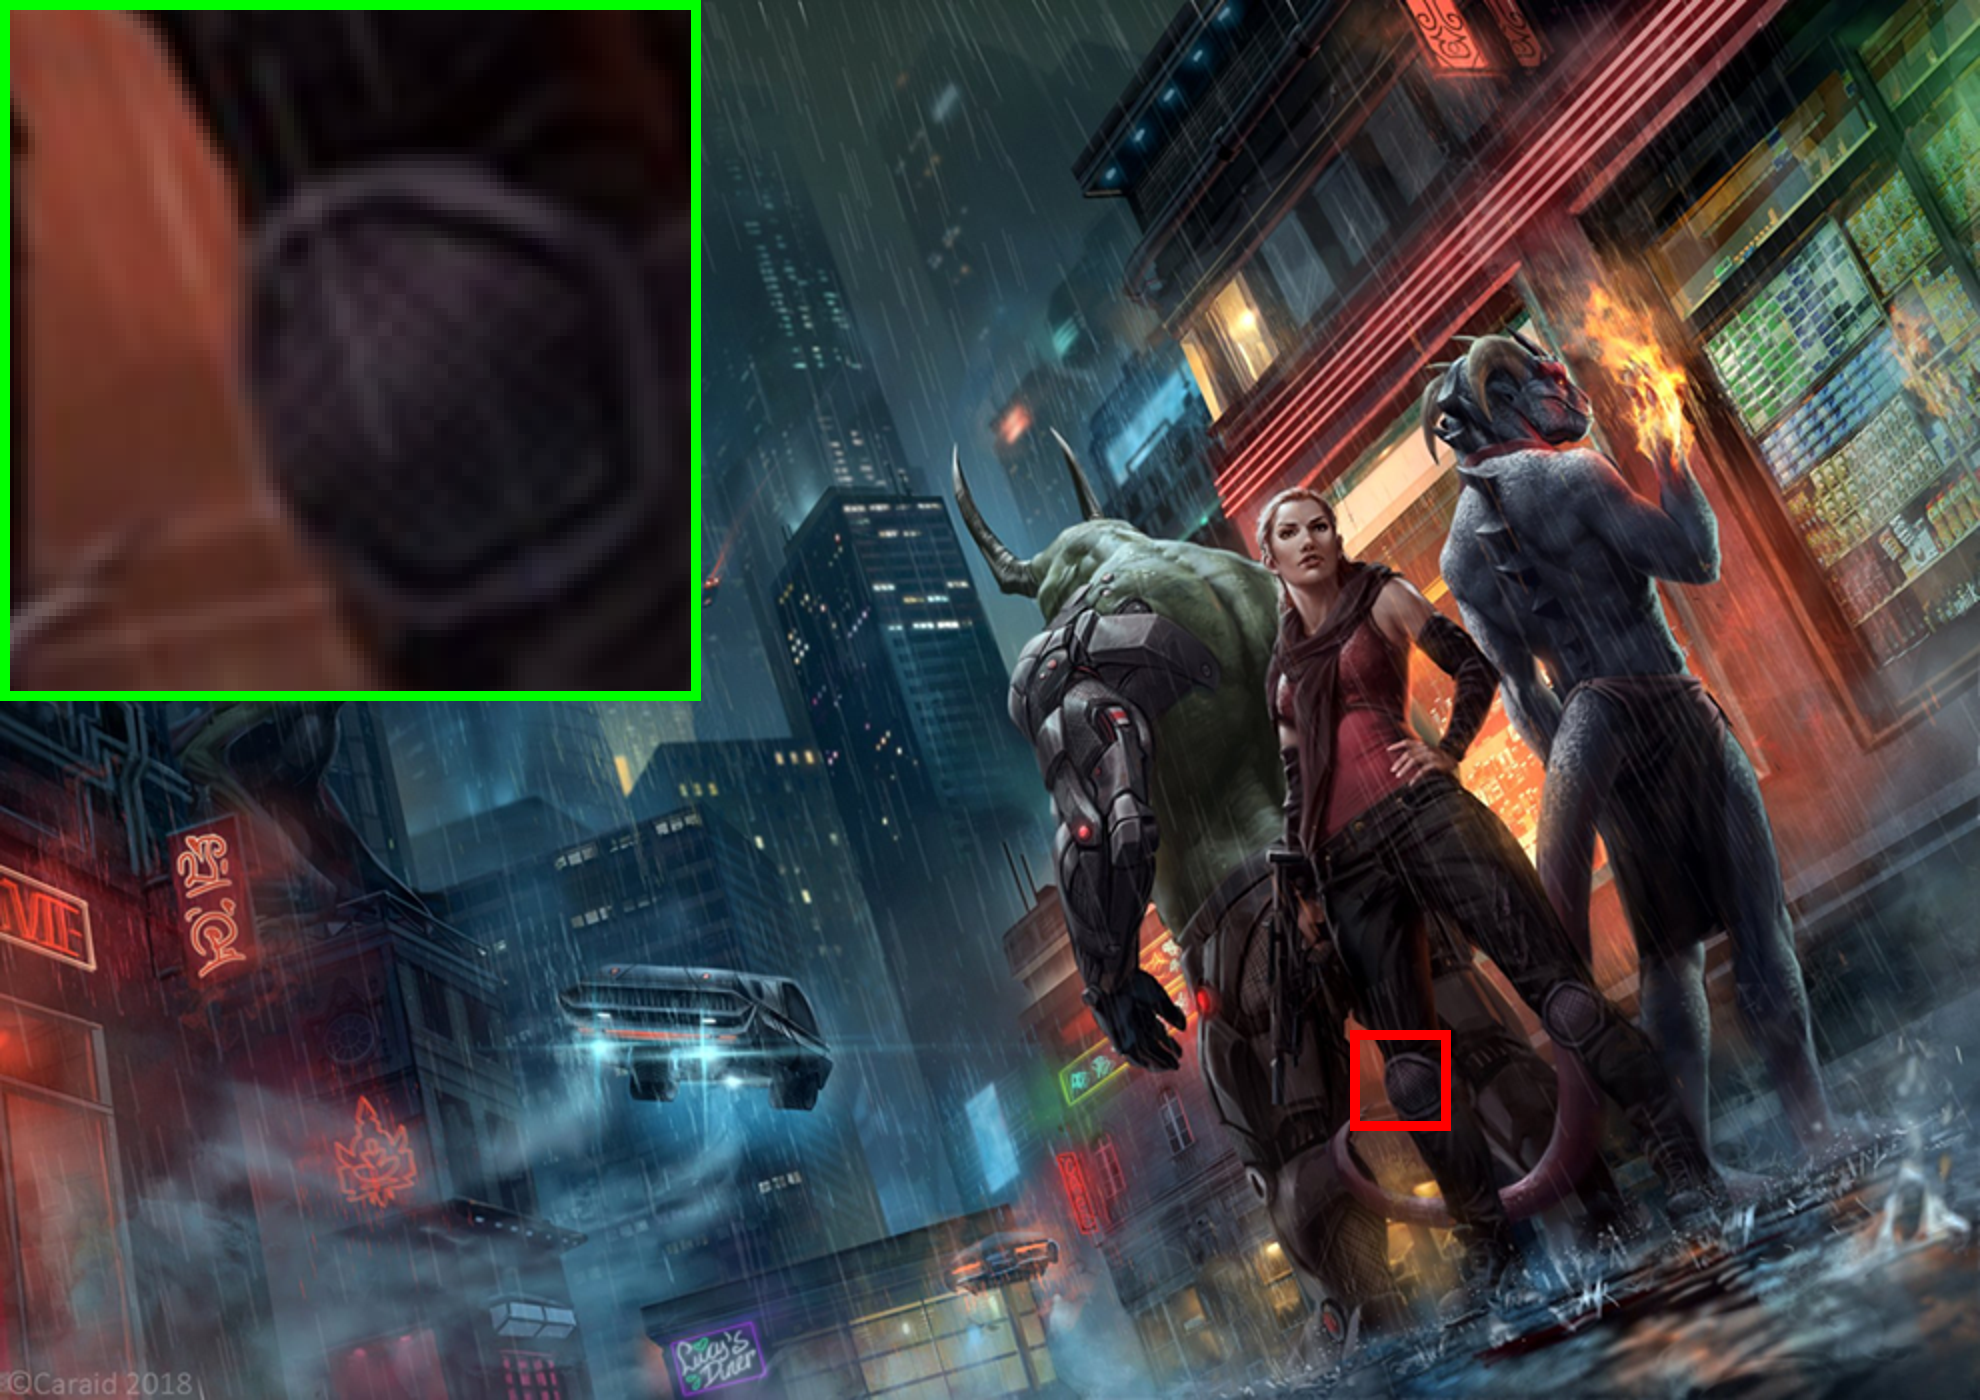
\includegraphics[width=\textwidth]{Figures/2X/Cyberpunk/Bicubic_Cyberpunk_GAUSS_0_comparison.png}
            \caption{Bicubic}
        \end{subfigure}
        \hfill
        \begin{subfigure}[b]{0.475\textwidth}  
            \centering 
            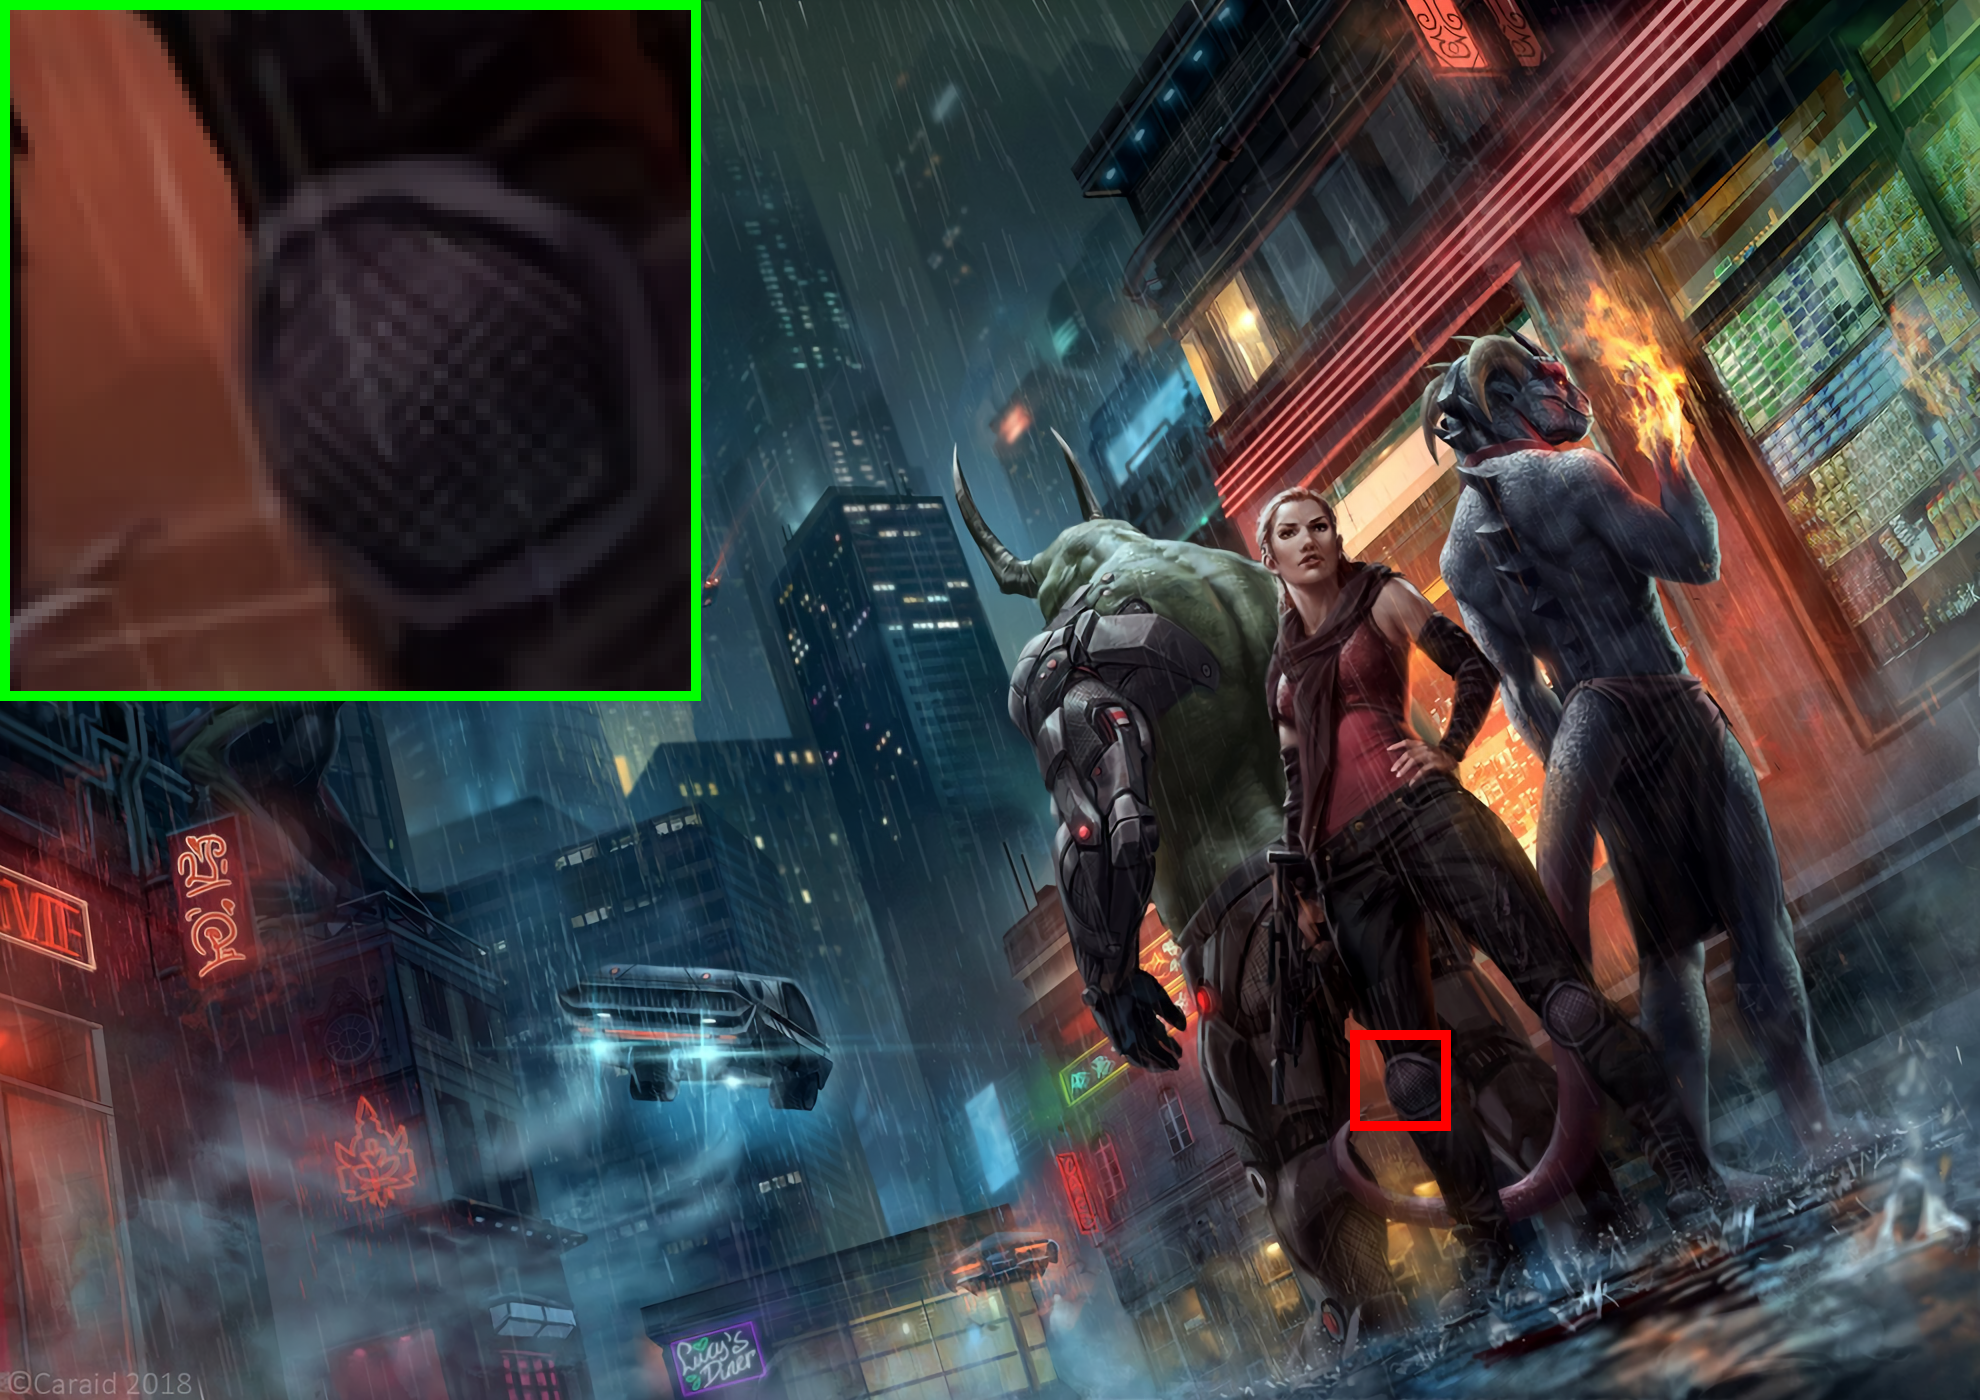
\includegraphics[width=\textwidth]{Figures/2X/Cyberpunk/EDSR_Cyberpunk_GAUSS_0_comparison.png}
            \caption{EDSR}     
        \end{subfigure}
        \vskip\baselineskip
        \begin{subfigure}[b]{0.475\textwidth}   
            \centering 
            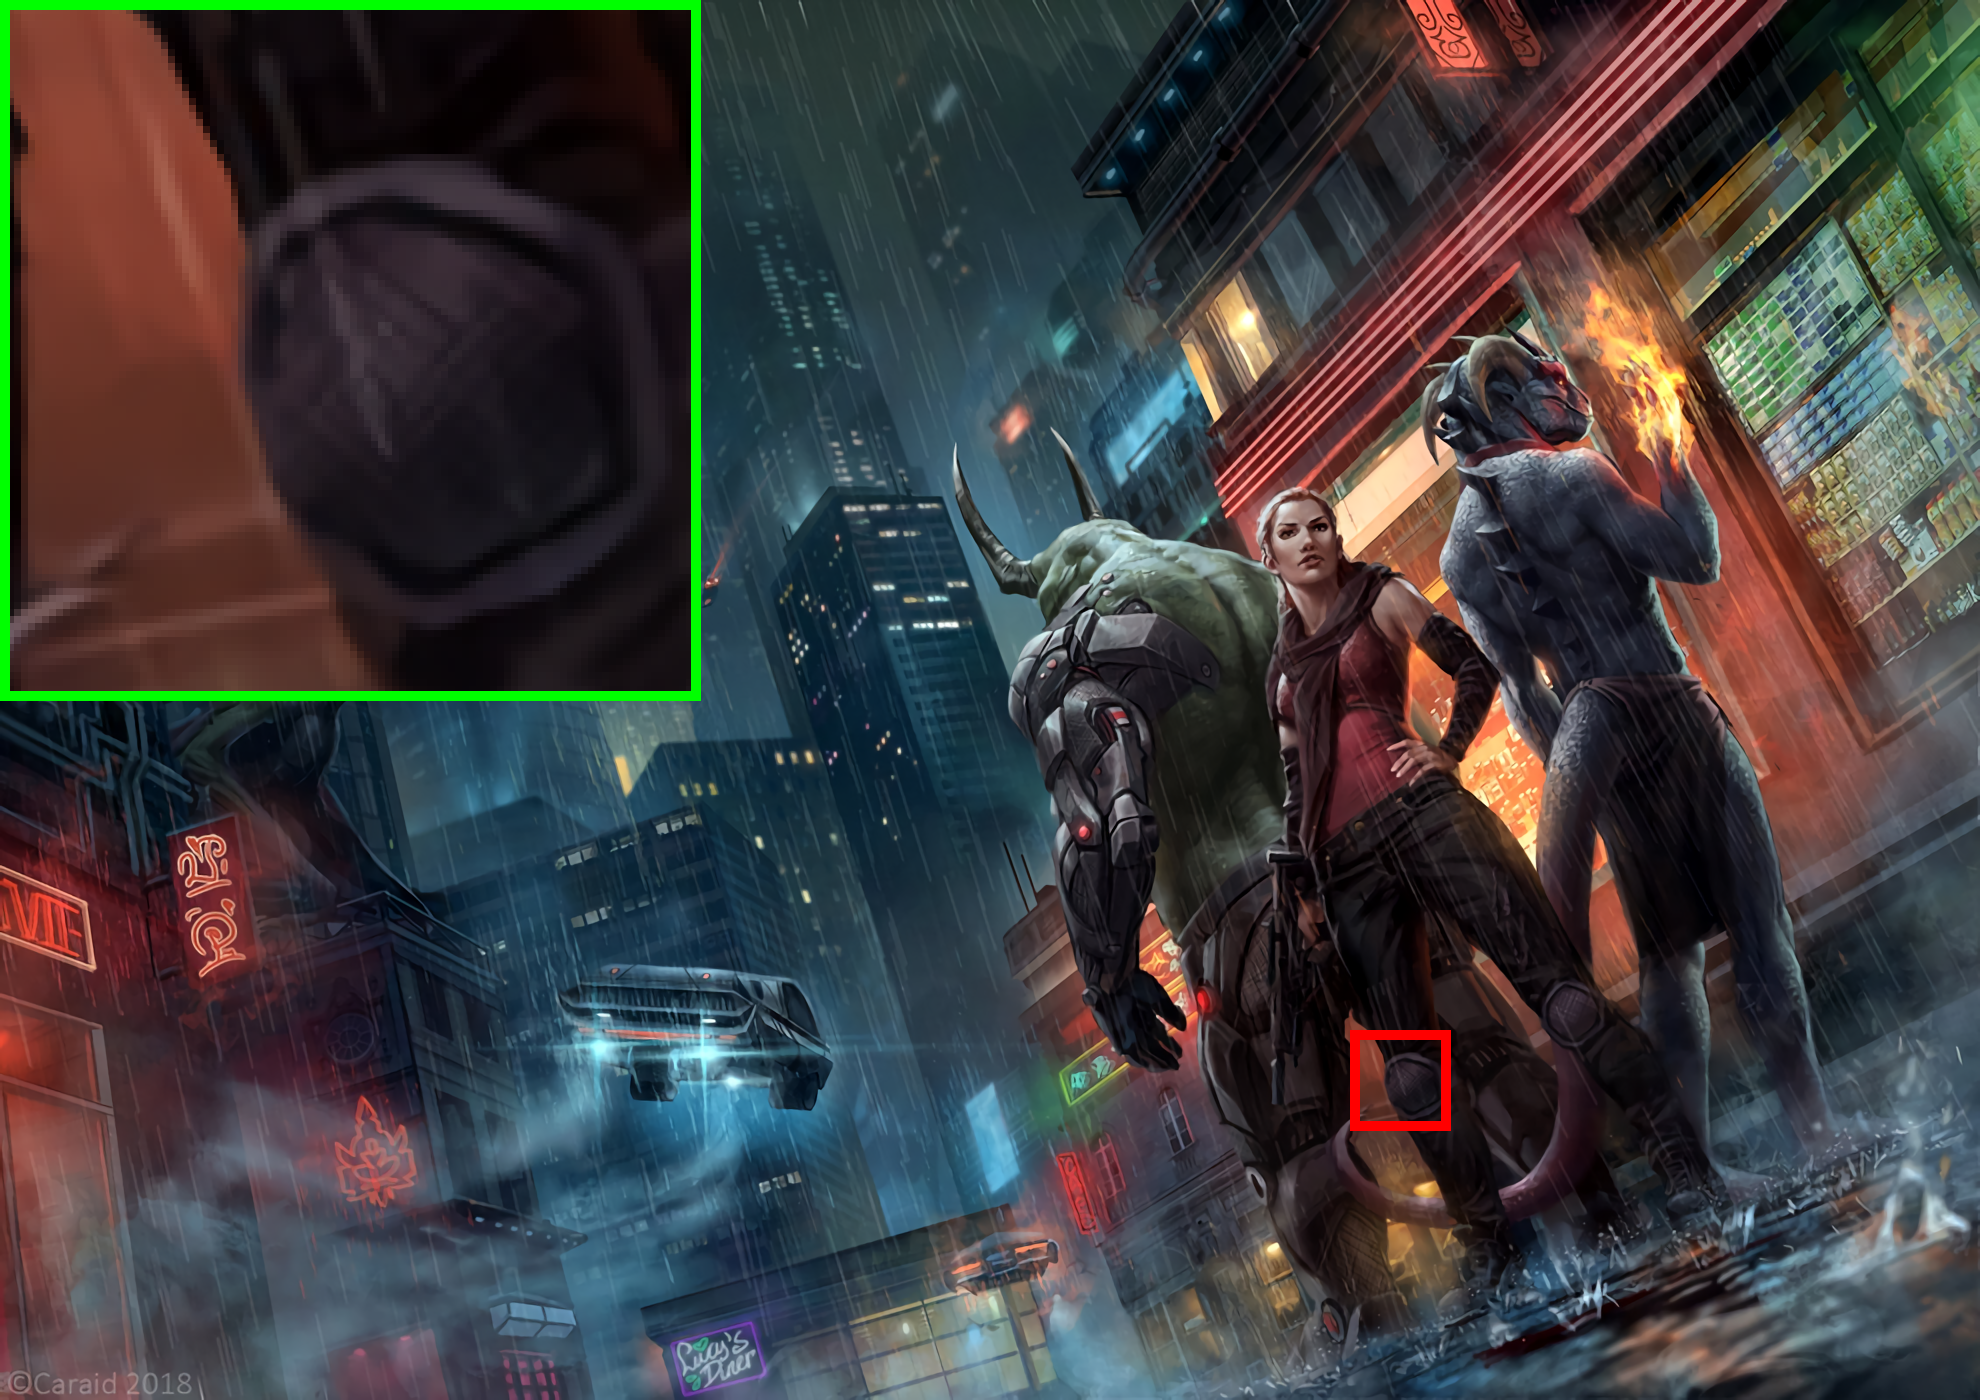
\includegraphics[width=\textwidth]{Figures/2X/Cyberpunk/Waifu2X_0_Cyberpunk_GAUSS_0_comparison.png}
            \caption{Waifu2x (level 0)}  
        \end{subfigure}
        \quad
        \begin{subfigure}[b]{0.475\textwidth}   
            \centering 
            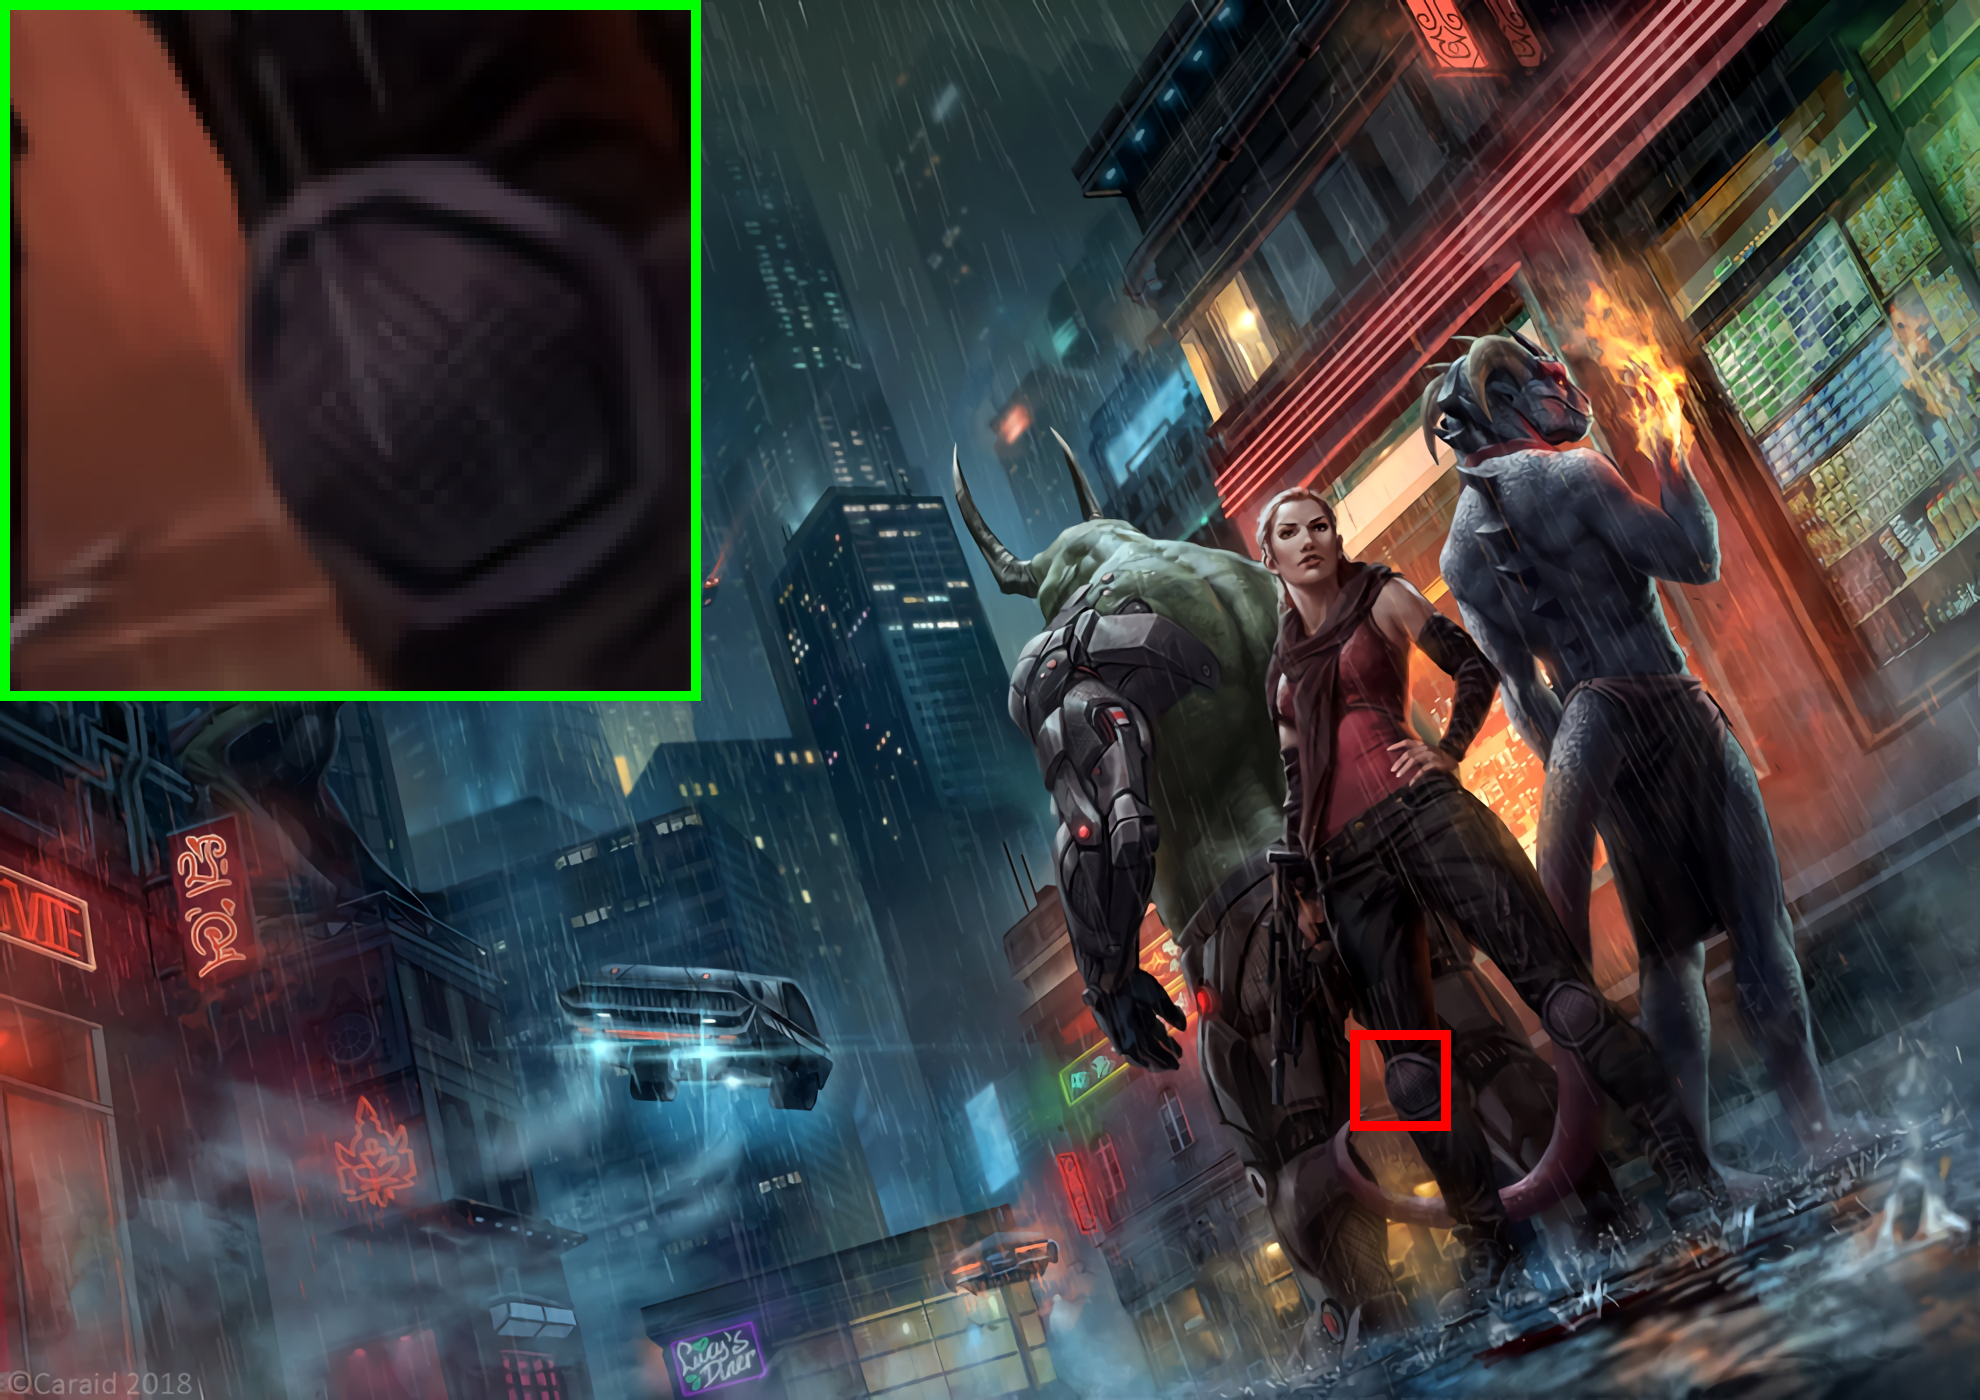
\includegraphics[width=\textwidth]{Figures/2X/Cyberpunk/Waifu2X_1_Cyberpunk_GAUSS_0_comparison.png}
            \caption{Waifu2x (level 1)}  
        \end{subfigure}
        \vskip\baselineskip
        \begin{subfigure}[b]{0.475\textwidth}   
            \centering 
            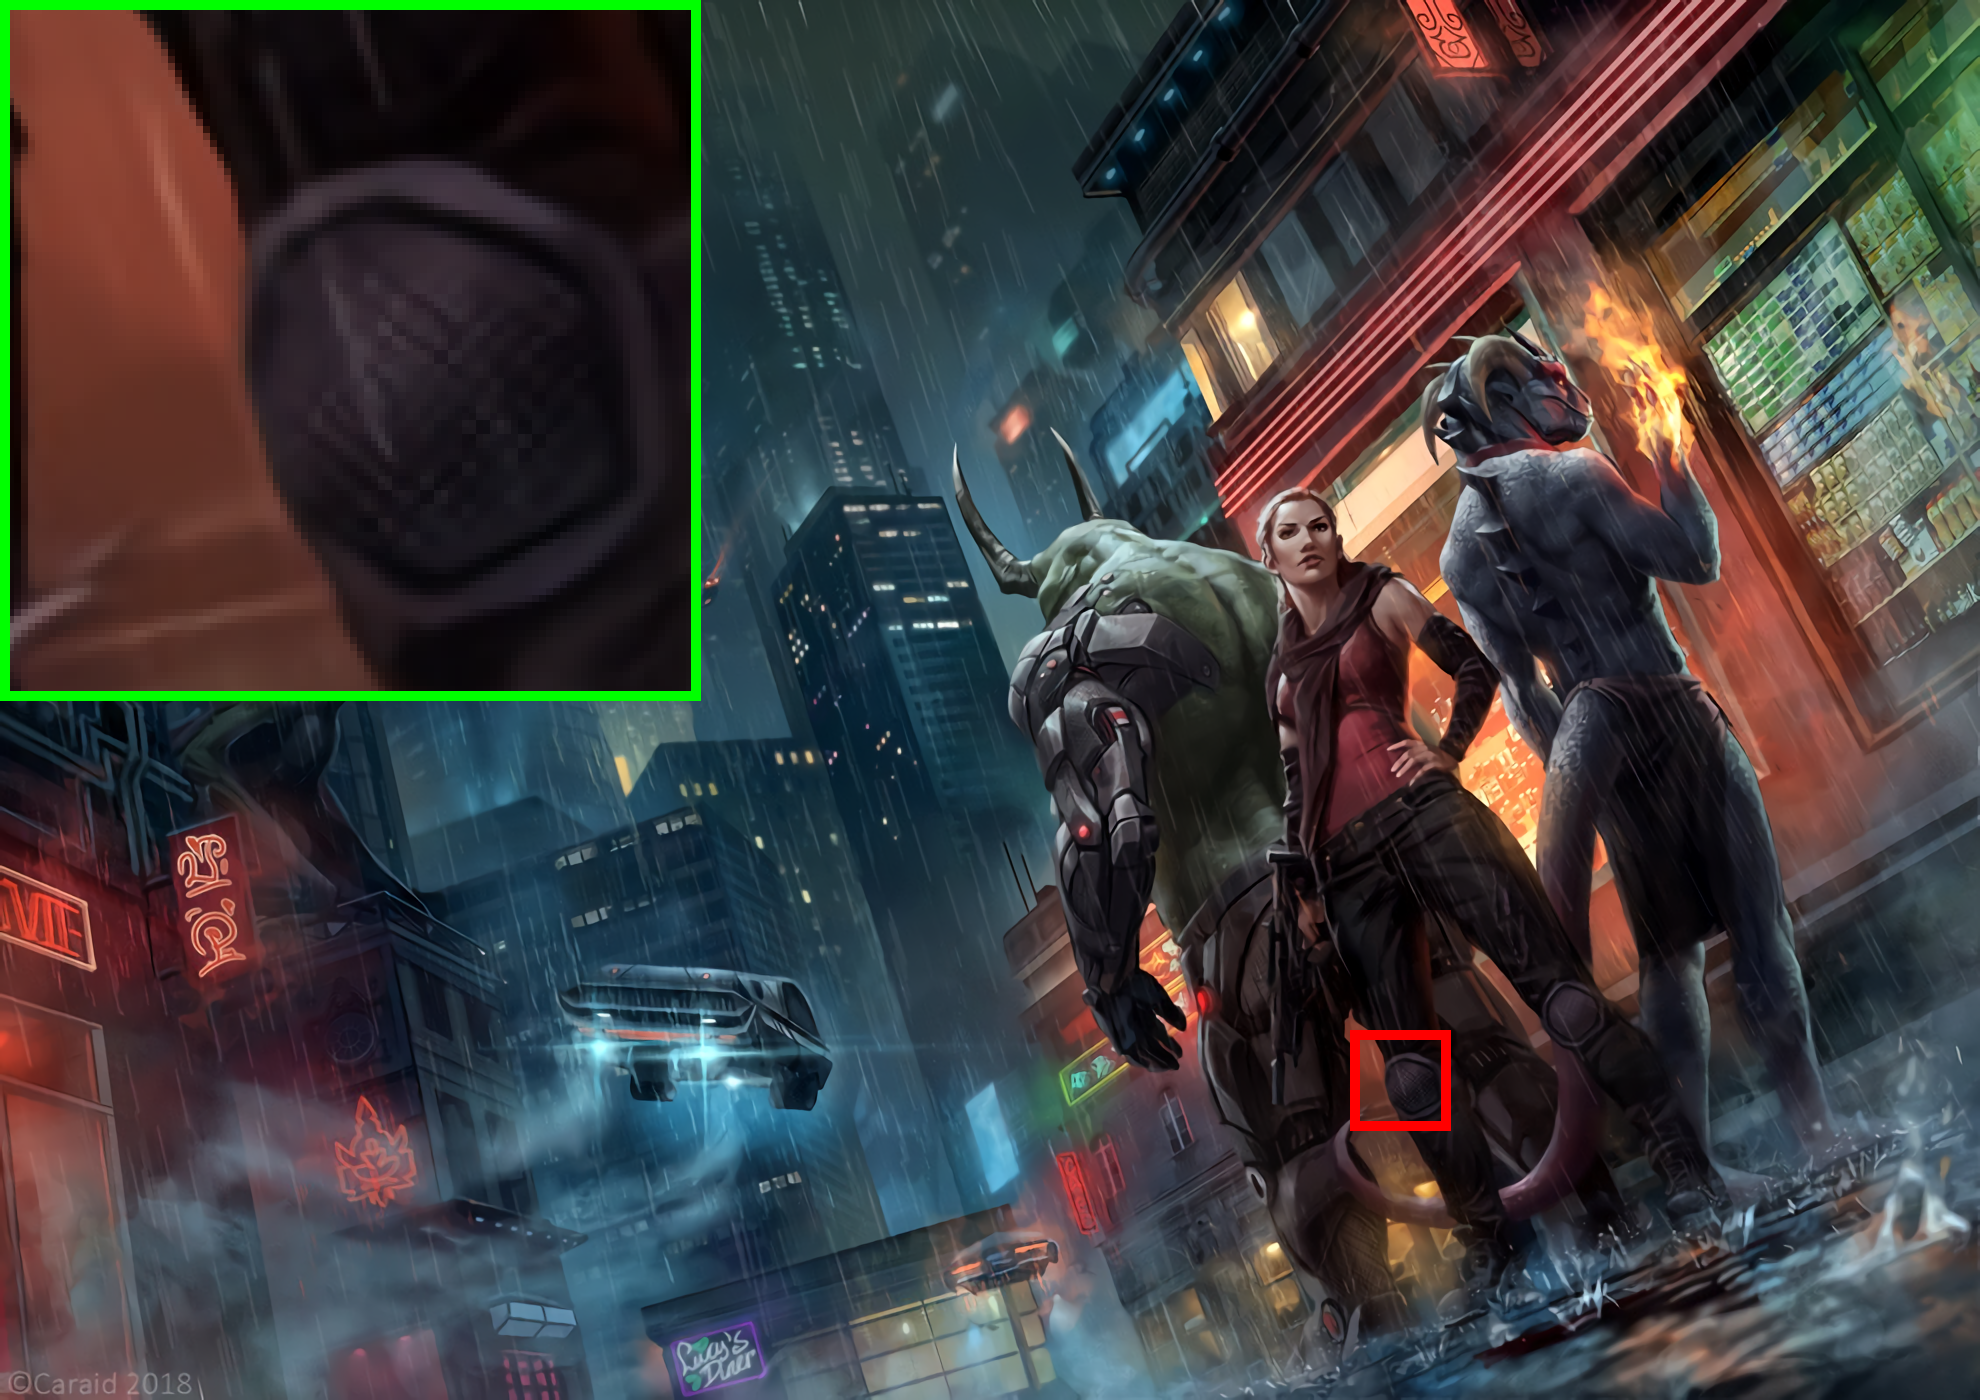
\includegraphics[width=\textwidth]{Figures/2X/Cyberpunk/Waifu2X_2_Cyberpunk_GAUSS_0_comparison.png}
            \caption{Waifu2x (level 2)}  
        \end{subfigure}
        \quad
        \begin{subfigure}[b]{0.475\textwidth}   
            \centering 
            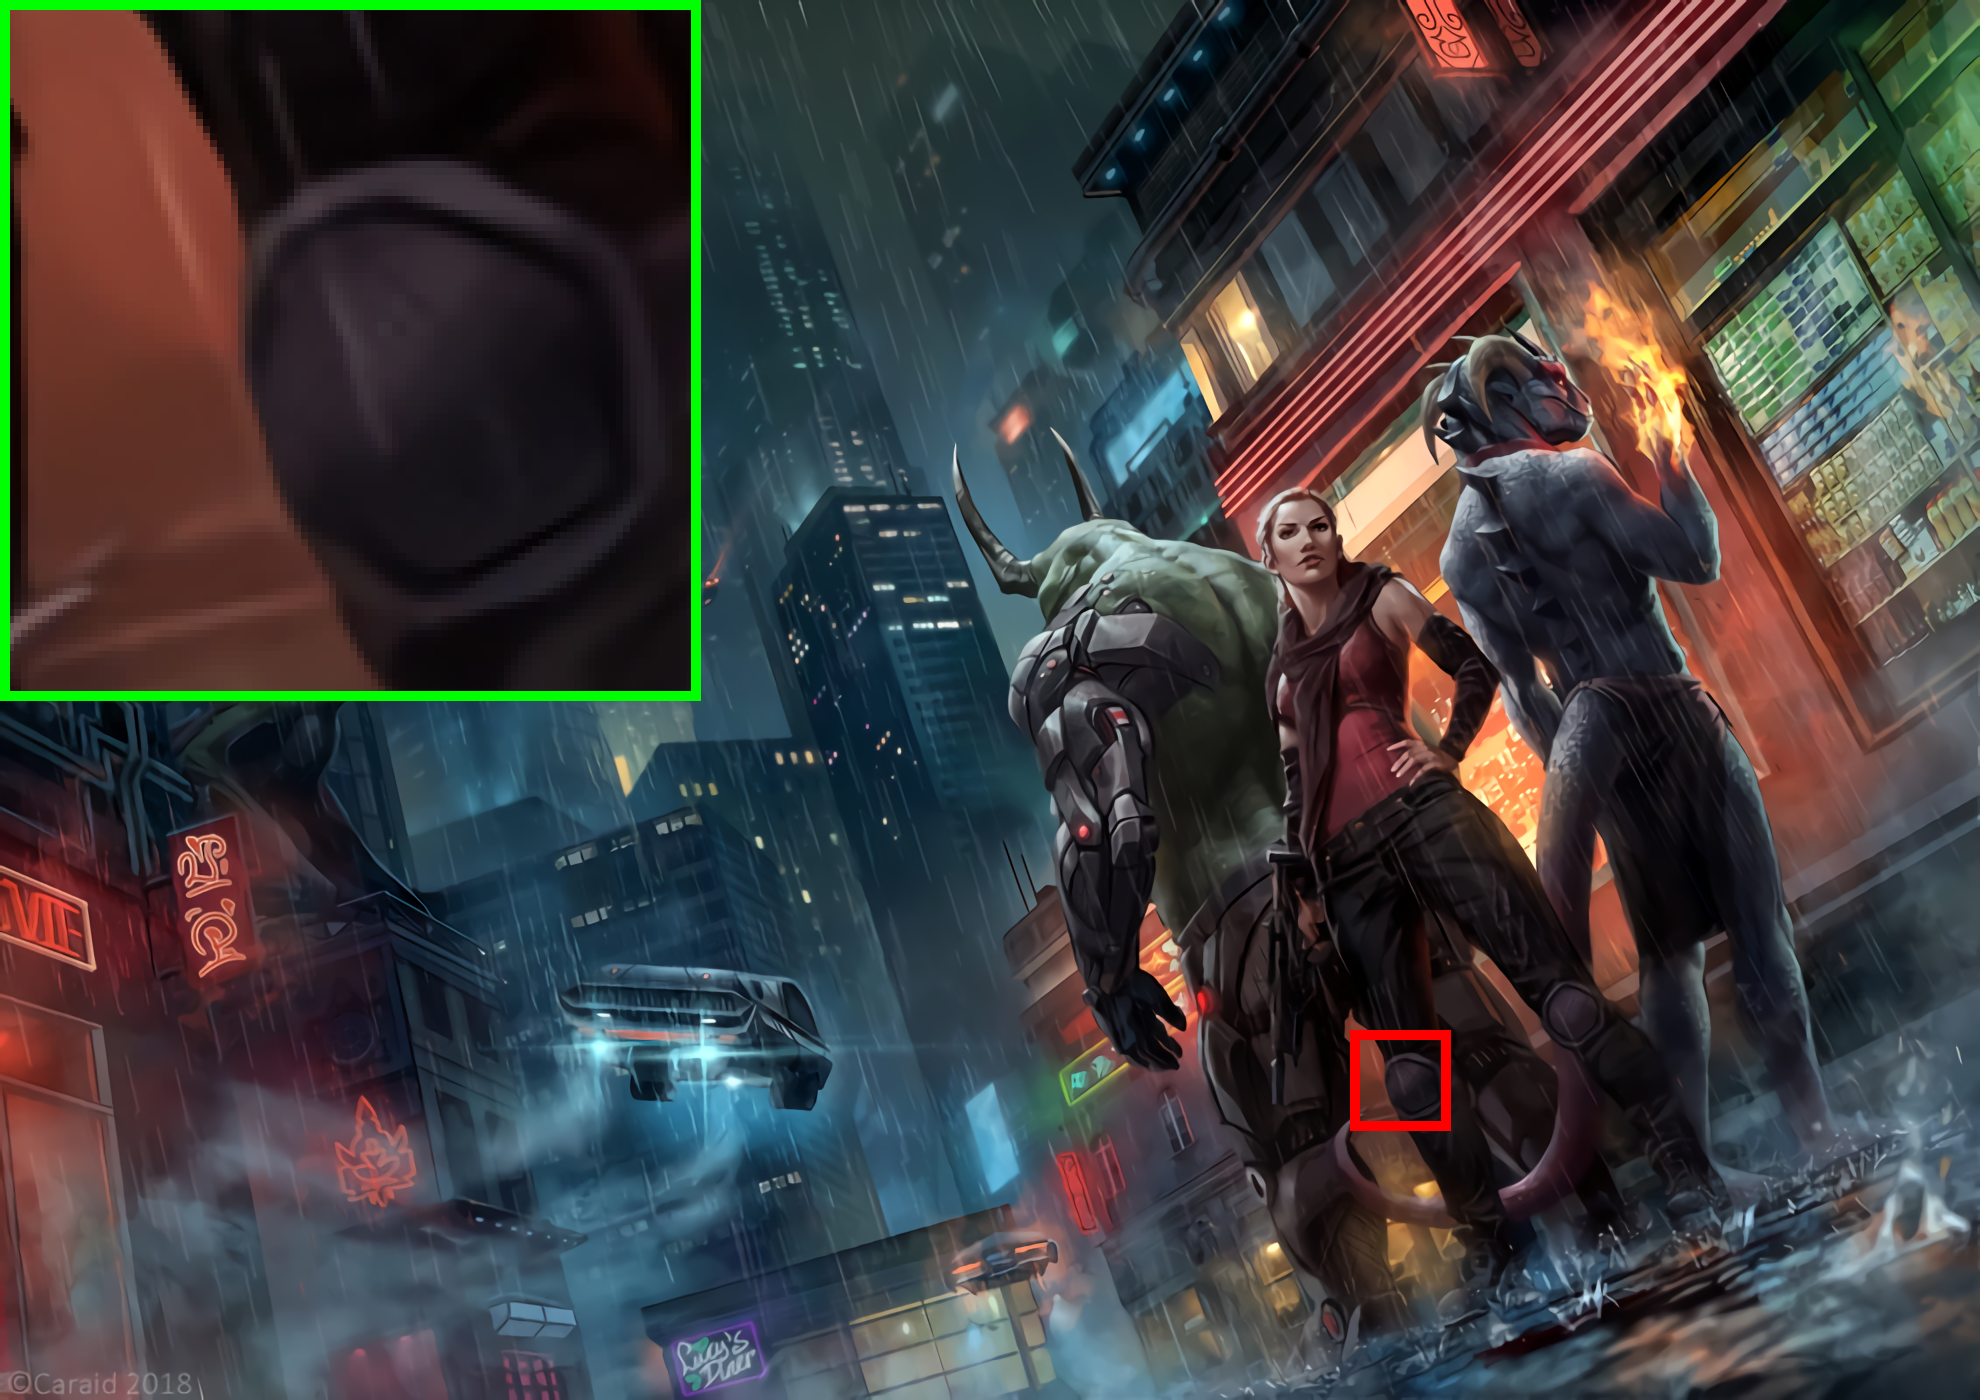
\includegraphics[width=\textwidth]{Figures/2X/Cyberpunk/Waifu2X_3_Cyberpunk_GAUSS_0_comparison.png}
            \caption{Waifu2x (level 3)}  
        \end{subfigure}
        \caption{Results of Waifu2x and my trained model on a clean version (GAUSS\_0) of one of the images}  
                \label{Cyberpunk_fig}
    \end{figure*}
    
    \begin{figure*}
        \centering
        \begin{subfigure}[b]{0.75\textwidth}
            \centering
            \includegraphics[width=\textwidth]{Figures/2X/Cyberpunk/be15968553390b112e723e8773910e11.png}
            \caption{High Resolution}
        \end{subfigure}
        \vskip\baselineskip
        \begin{subfigure}[b]{0.475\textwidth}
            \centering
            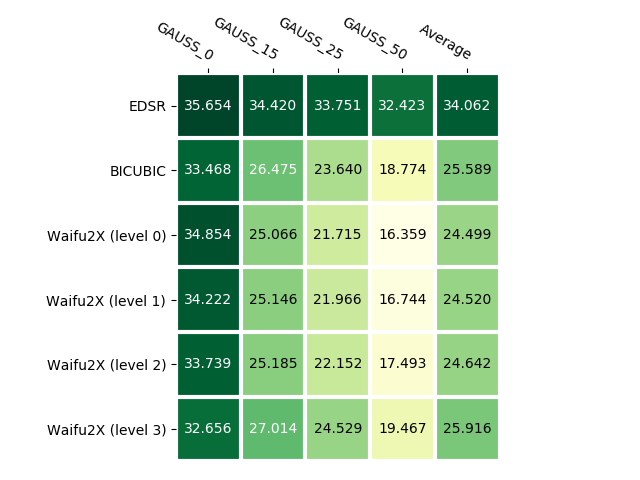
\includegraphics[width=\textwidth]{Figures/2X/Cyberpunk/PSNR_GAUSS_Cyberpunk.png}
            \caption{PSNR results with gaussian noise}
        \end{subfigure}
        \hfill
        \begin{subfigure}[b]{0.475\textwidth}  
            \centering 
            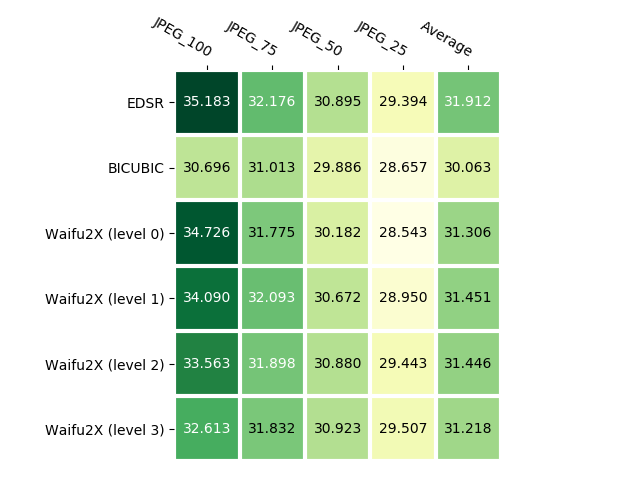
\includegraphics[width=\textwidth]{Figures/2X/Cyberpunk/PSNR_JPEG_Cyberpunk.png}
            \caption{PSNR results with JPEG noise}
        \end{subfigure}
        \vskip\baselineskip
        \begin{subfigure}[b]{0.475\textwidth}   
            \centering 
            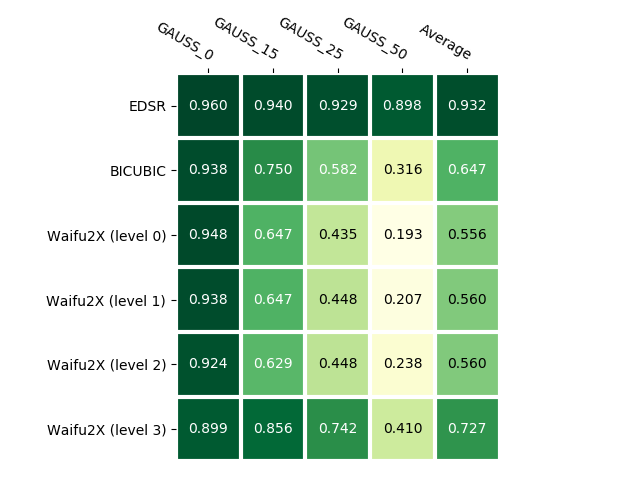
\includegraphics[width=\textwidth]{Figures/2X/Cyberpunk/SSIM_GAUSS_Cyberpunk.png}
            \caption{SSIM results with gaussian noise}
        \end{subfigure}
        \quad
        \begin{subfigure}[b]{0.475\textwidth}   
            \centering 
            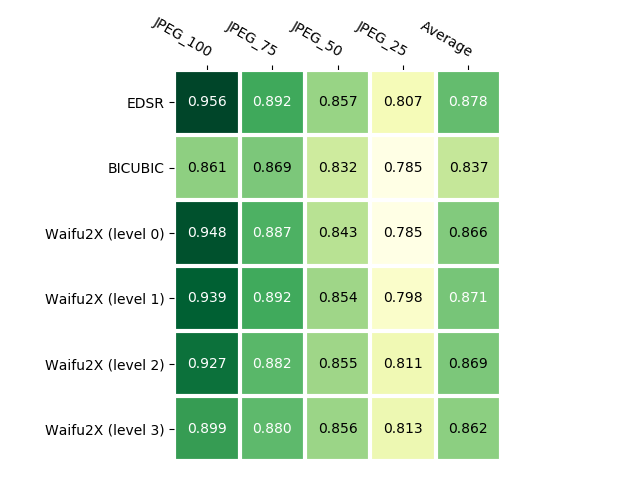
\includegraphics[width=\textwidth]{Figures/2X/Cyberpunk/SSIM_JPEG_Cyberpunk.png}
            \caption{SSIM results with JPEG noise}
        \end{subfigure}
        \caption{PSNR and SSIM results on the shown image}
    \end{figure*}
    
    \begin{figure*}
        \centering
        \begin{subfigure}[b]{0.75\textwidth}
            \centering
            \includegraphics[width=\textwidth]{Figures/2X/Tiger/image.png}
            \caption{High Resolution}
        \end{subfigure}
        \vskip\baselineskip
        \begin{subfigure}[b]{0.475\textwidth}
            \centering
            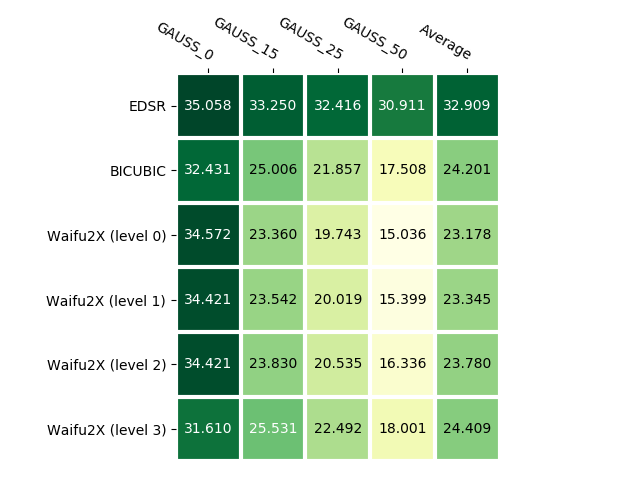
\includegraphics[width=\textwidth]{Figures/2X/Tiger/PSNR_GAUSS.png}
            \caption{PSNR results with gaussian noise}
        \end{subfigure}
        \hfill
        \begin{subfigure}[b]{0.475\textwidth}  
            \centering 
            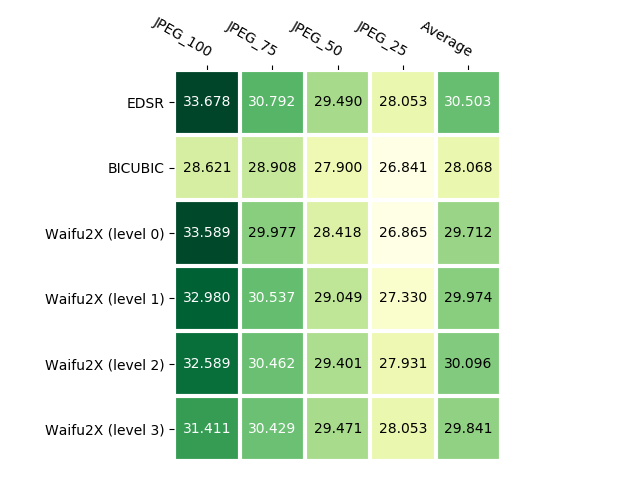
\includegraphics[width=\textwidth]{Figures/2X/Tiger/PSNR_JPEG.png}
            \caption{PSNR results with JPEG noise}
        \end{subfigure}
        \vskip\baselineskip
        \begin{subfigure}[b]{0.475\textwidth}   
            \centering 
            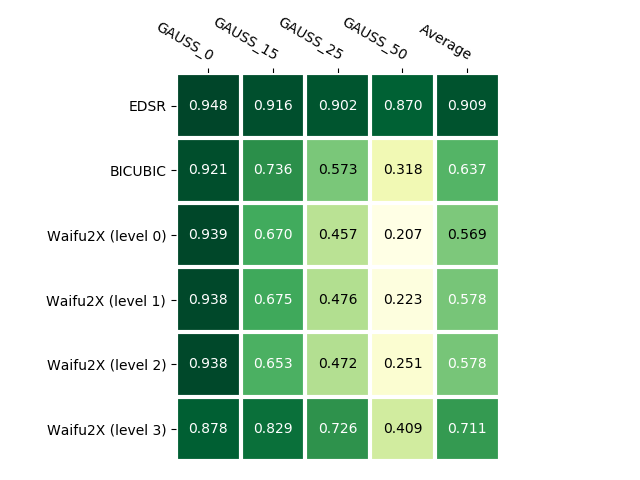
\includegraphics[width=\textwidth]{Figures/2X/Tiger/SSIM_GAUSS.png}
            \caption{SSIM results with gaussian noise}
        \end{subfigure}
        \quad
        \begin{subfigure}[b]{0.475\textwidth}   
            \centering 
            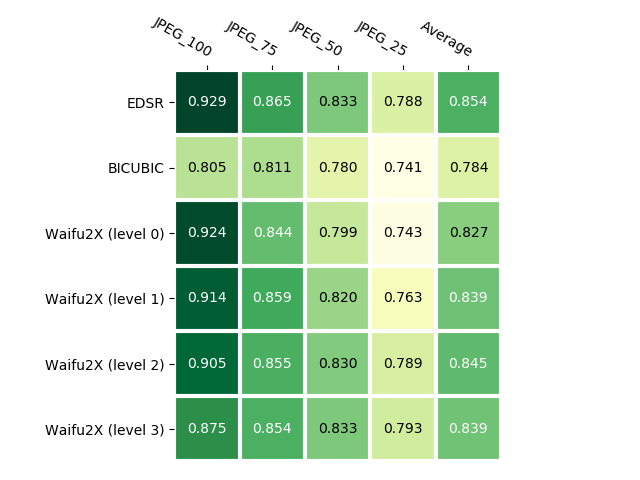
\includegraphics[width=\textwidth]{Figures/2X/Tiger/SSIM_JPEG.png}
            \caption{SSIM results with JPEG noise}
        \end{subfigure}
        \caption{PSNR and SSIM results on the shown image}
    \end{figure*}
    
        \begin{figure*}
        \centering
        \begin{subfigure}[b]{0.75\textwidth}
            \centering
            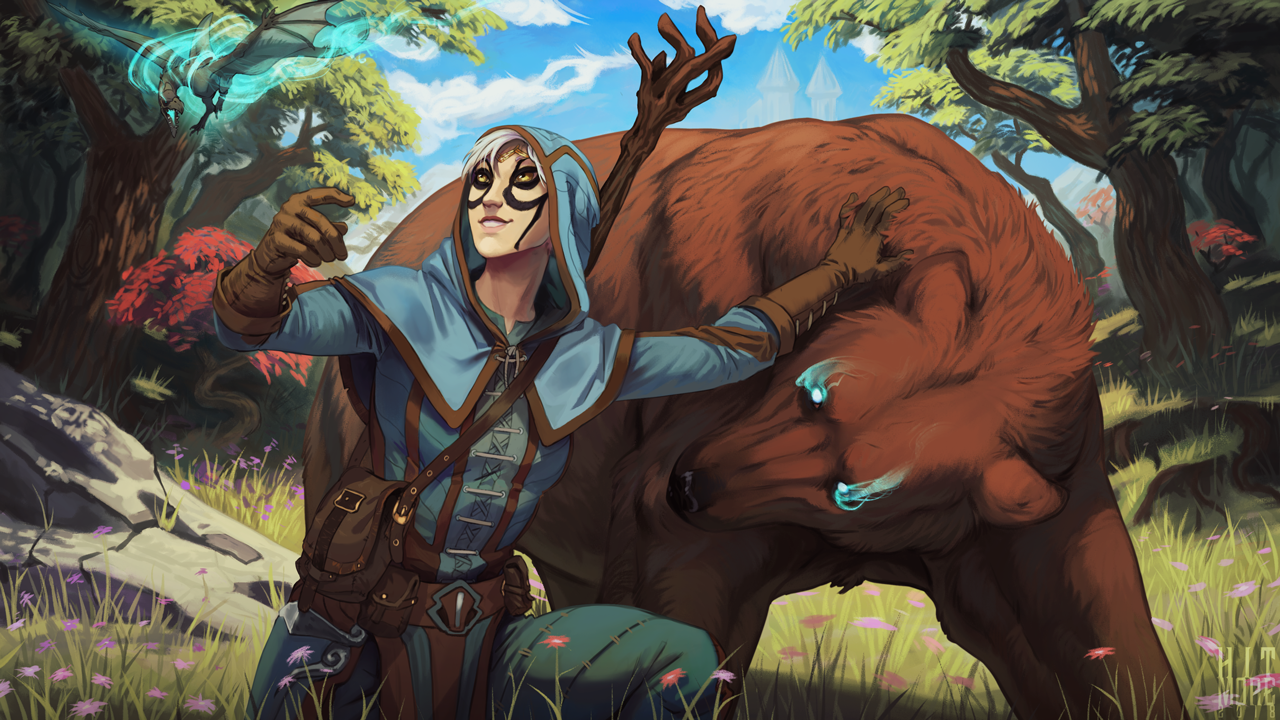
\includegraphics[width=\textwidth]{Figures/2X/Bear/image.png}
            \caption{High Resolution}
        \end{subfigure}
        \vskip\baselineskip
        \begin{subfigure}[b]{0.475\textwidth}
            \centering
            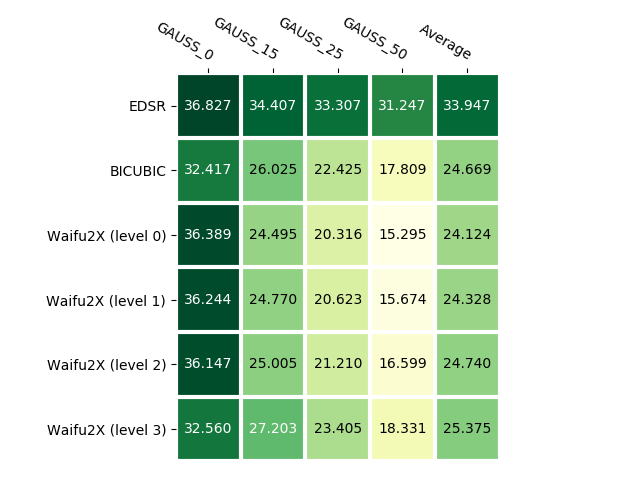
\includegraphics[width=\textwidth]{Figures/2X/Bear/PSNR_GAUSS.png}
            \caption{PSNR results with gaussian noise}
        \end{subfigure}
        \hfill
        \begin{subfigure}[b]{0.475\textwidth}  
            \centering 
            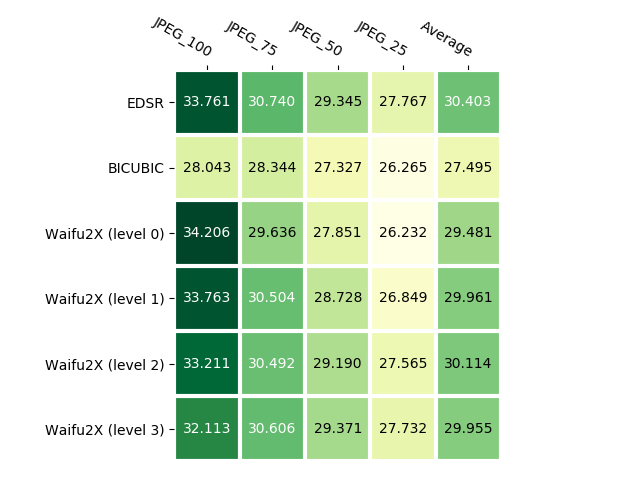
\includegraphics[width=\textwidth]{Figures/2X/Bear/PSNR_JPEG.png}
            \caption{PSNR results with JPEG noise}
        \end{subfigure}
        \vskip\baselineskip
        \begin{subfigure}[b]{0.475\textwidth}   
            \centering 
            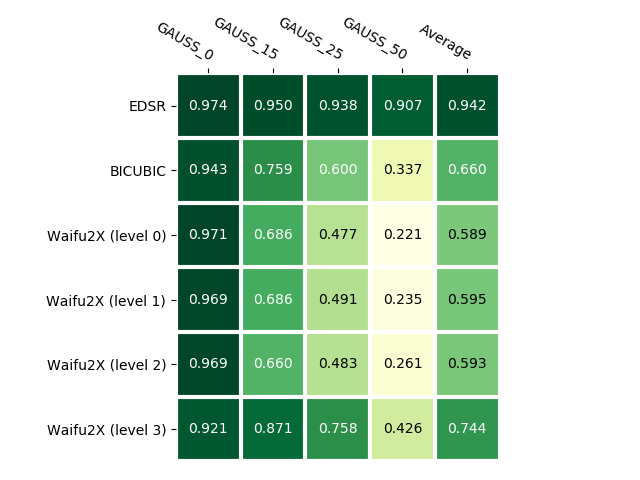
\includegraphics[width=\textwidth]{Figures/2X/Bear/SSIM_GAUSS.png}
            \caption{SSIM results with gaussian noise}
        \end{subfigure}
        \quad
        \begin{subfigure}[b]{0.475\textwidth}   
            \centering 
            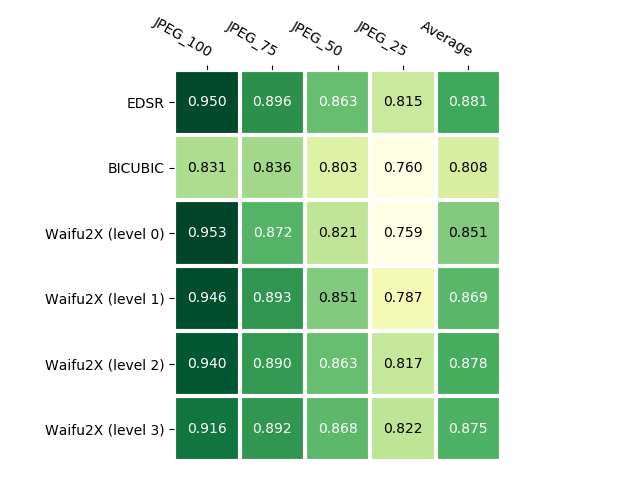
\includegraphics[width=\textwidth]{Figures/2X/Bear/SSIM_JPEG.png}
            \caption{SSIM results with JPEG noise}
        \end{subfigure}
        \caption{PSNR and SSIM results on the shown image}
    \end{figure*}
    
        \begin{figure*}
        \centering
        \begin{subfigure}[b]{0.75\textwidth}
            \centering
            \includegraphics[width=\textwidth]{Figures/2X/Catch/image.png}
            \caption{High Resolution}
        \end{subfigure}
        \vskip\baselineskip
        \begin{subfigure}[b]{0.475\textwidth}
            \centering
            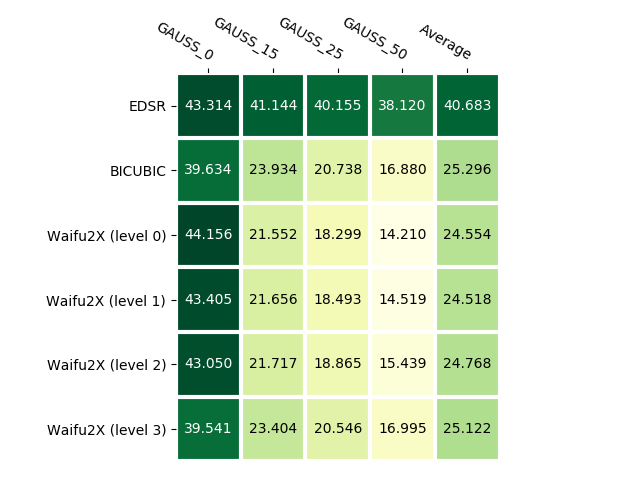
\includegraphics[width=\textwidth]{Figures/2X/Catch/PSNR_GAUSS.png}
            \caption{PSNR results with gaussian noise}
        \end{subfigure}
        \hfill
        \begin{subfigure}[b]{0.475\textwidth}  
            \centering 
            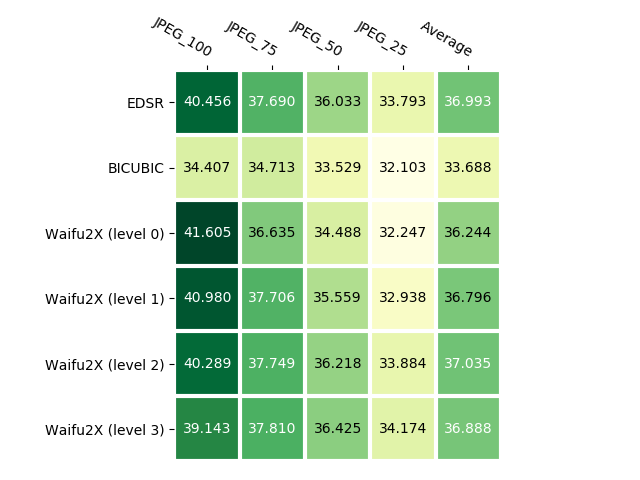
\includegraphics[width=\textwidth]{Figures/2X/Catch/PSNR_JPEG.png}
            \caption{PSNR results with JPEG noise}
        \end{subfigure}
        \vskip\baselineskip
        \begin{subfigure}[b]{0.475\textwidth}   
            \centering 
            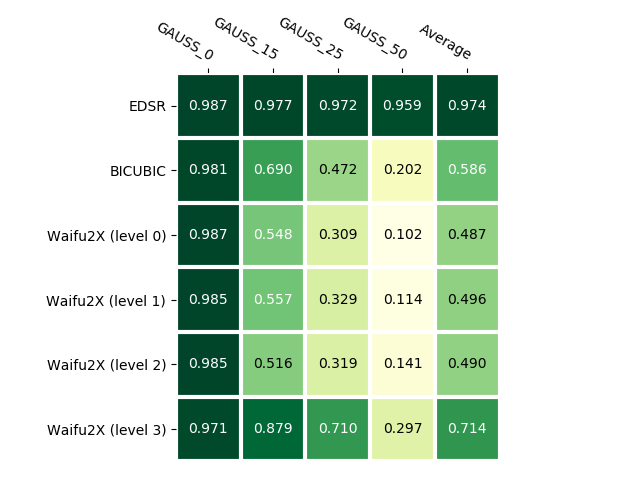
\includegraphics[width=\textwidth]{Figures/2X/Catch/SSIM_GAUSS.png}
            \caption{SSIM results with gaussian noise}
        \end{subfigure}
        \quad
        \begin{subfigure}[b]{0.475\textwidth}   
            \centering 
            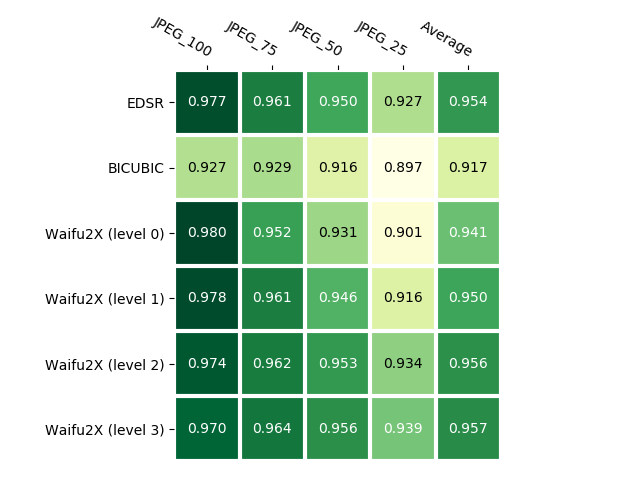
\includegraphics[width=\textwidth]{Figures/2X/Catch/SSIM_JPEG.png}
            \caption{SSIM results with JPEG noise}
        \end{subfigure}
        \caption{PSNR and SSIM results on the shown image}
    \end{figure*}
    
            \begin{figure*}
        \centering
        \begin{subfigure}[b]{0.75\textwidth}
            \centering
            \includegraphics[width=\textwidth]{Figures/2X/Coffee/image.png}
            \caption{High Resolution}
        \end{subfigure}
        \vskip\baselineskip
        \begin{subfigure}[b]{0.475\textwidth}
            \centering
            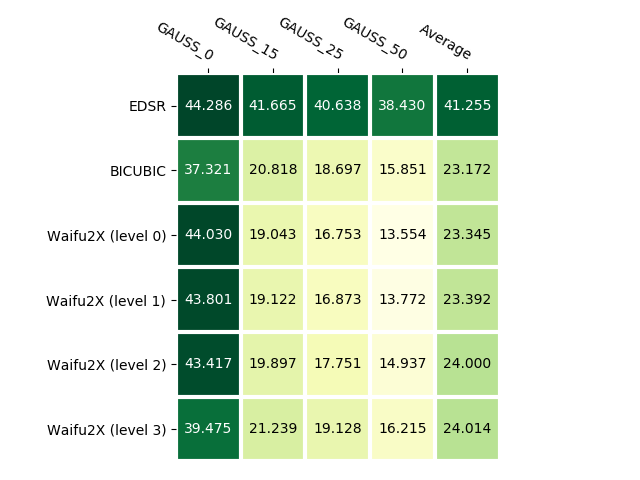
\includegraphics[width=\textwidth]{Figures/2X/Coffee/PSNR_GAUSS.png}
            \caption{PSNR results with gaussian noise}
        \end{subfigure}
        \hfill
        \begin{subfigure}[b]{0.475\textwidth}  
            \centering 
            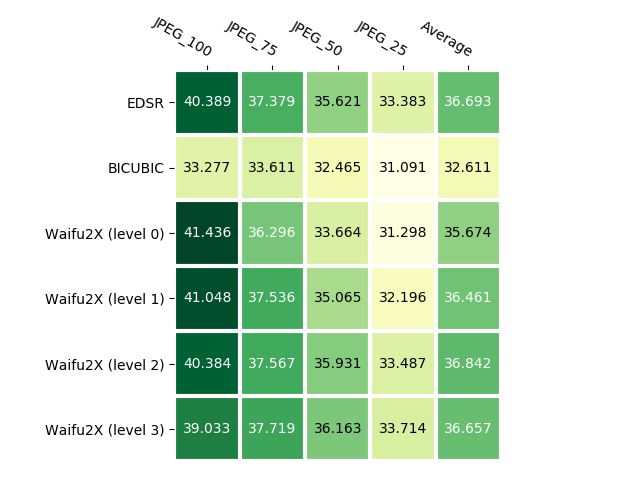
\includegraphics[width=\textwidth]{Figures/2X/Coffee/PSNR_JPEG.png}
            \caption{PSNR results with JPEG noise}
        \end{subfigure}
        \vskip\baselineskip
        \begin{subfigure}[b]{0.475\textwidth}   
            \centering 
            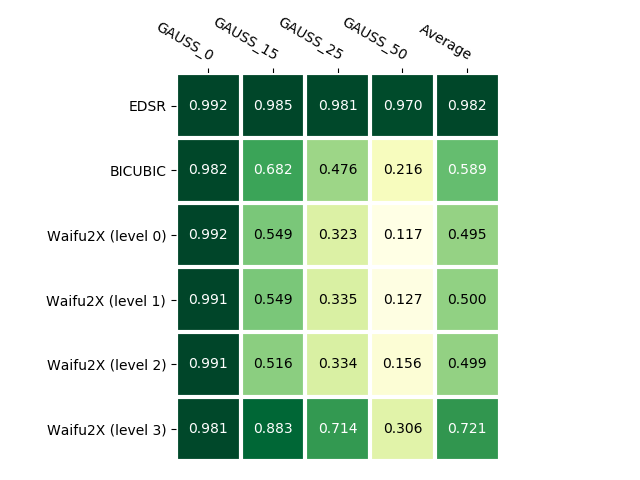
\includegraphics[width=\textwidth]{Figures/2X/Coffee/SSIM_GAUSS.png}
            \caption{SSIM results with gaussian noise}
        \end{subfigure}
        \quad
        \begin{subfigure}[b]{0.475\textwidth}   
            \centering 
            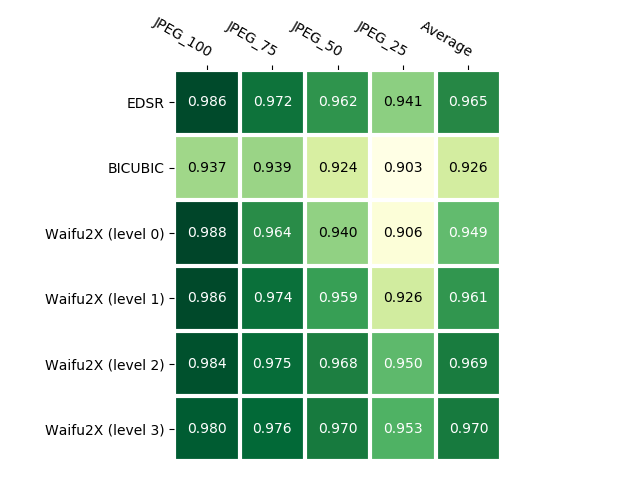
\includegraphics[width=\textwidth]{Figures/2X/Coffee/SSIM_JPEG.png}
            \caption{SSIM results with JPEG noise}
        \end{subfigure}
        \caption{PSNR and SSIM results on the shown image}
    \end{figure*}
    
            \begin{figure*}
        \centering
        \begin{subfigure}[b]{0.75\textwidth}
            \centering
            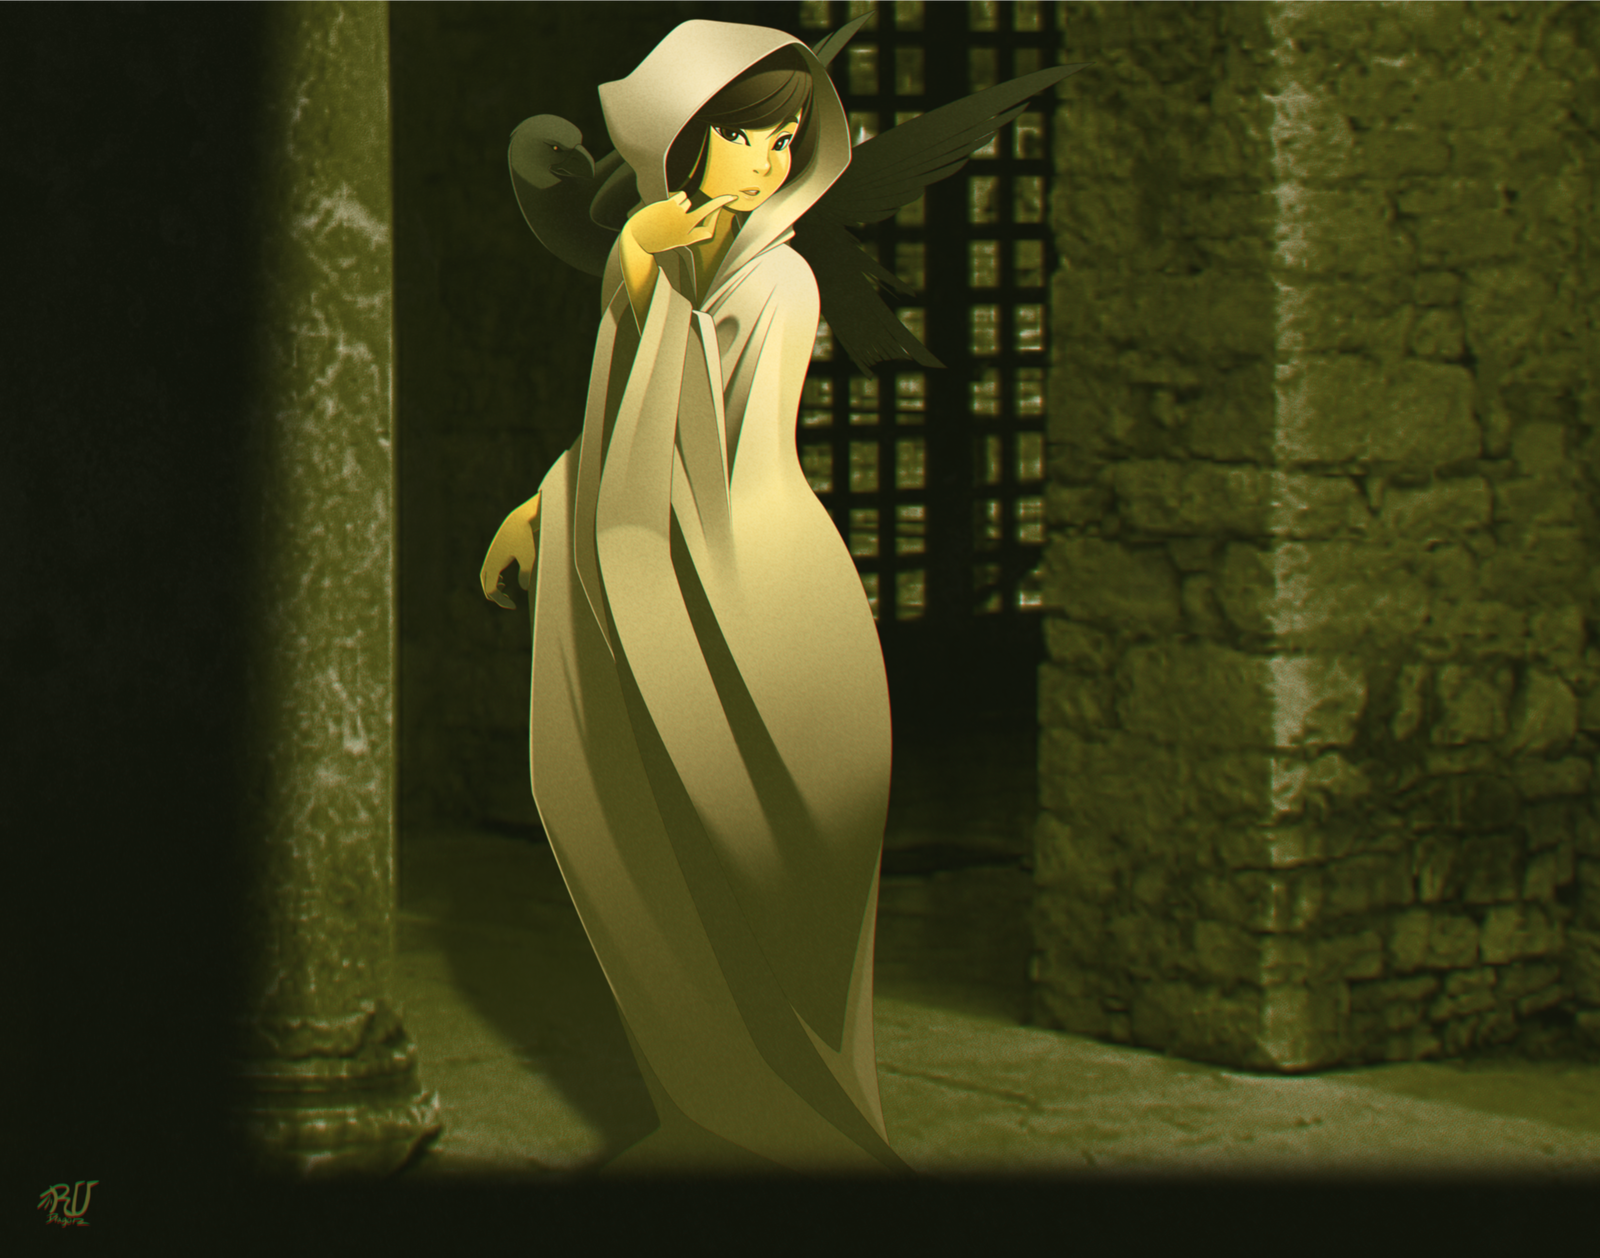
\includegraphics[width=\textwidth]{Figures/2X/Crow/image.png}
            \caption{High Resolution}
        \end{subfigure}
        \vskip\baselineskip
        \begin{subfigure}[b]{0.475\textwidth}
            \centering
            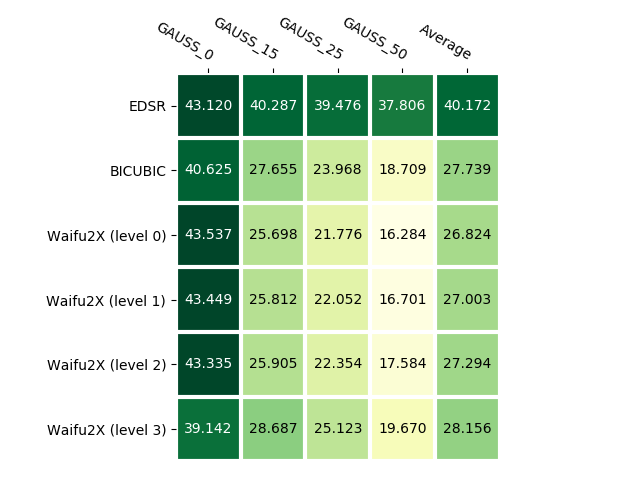
\includegraphics[width=\textwidth]{Figures/2X/Crow/PSNR_GAUSS.png}
            \caption{PSNR results with gaussian noise}
        \end{subfigure}
        \hfill
        \begin{subfigure}[b]{0.475\textwidth}  
            \centering 
            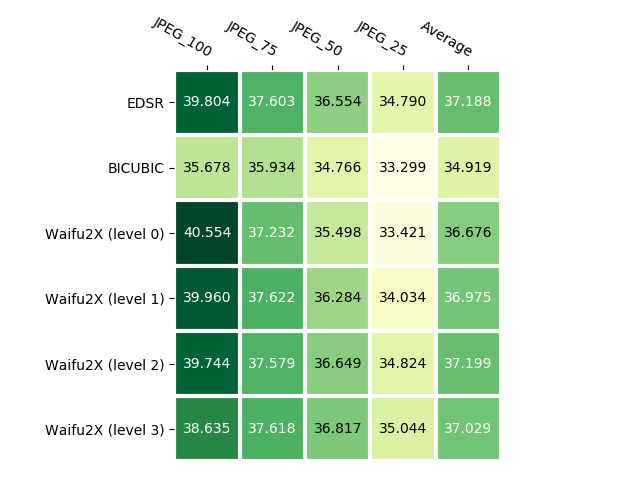
\includegraphics[width=\textwidth]{Figures/2X/Crow/PSNR_JPEG.png}
            \caption{PSNR results with JPEG noise}
        \end{subfigure}
        \vskip\baselineskip
        \begin{subfigure}[b]{0.475\textwidth}   
            \centering 
            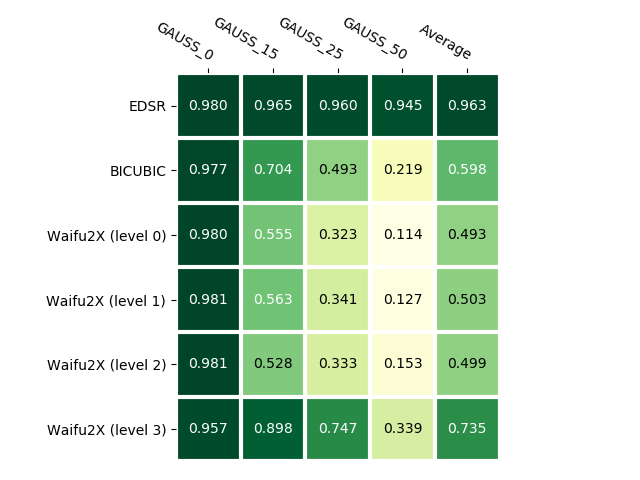
\includegraphics[width=\textwidth]{Figures/2X/Crow/SSIM_GAUSS.png}
            \caption{SSIM results with gaussian noise}
        \end{subfigure}
        \quad
        \begin{subfigure}[b]{0.475\textwidth}   
            \centering 
            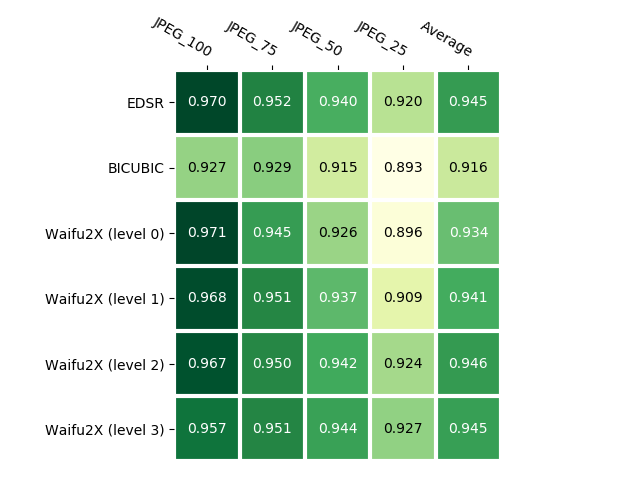
\includegraphics[width=\textwidth]{Figures/2X/Crow/SSIM_JPEG.png}
            \caption{SSIM results with JPEG noise}
        \end{subfigure}
        \caption{PSNR and SSIM results on the shown image}
    \end{figure*}
    
            \begin{figure*}
        \centering
        \begin{subfigure}[b]{0.75\textwidth}
            \centering
            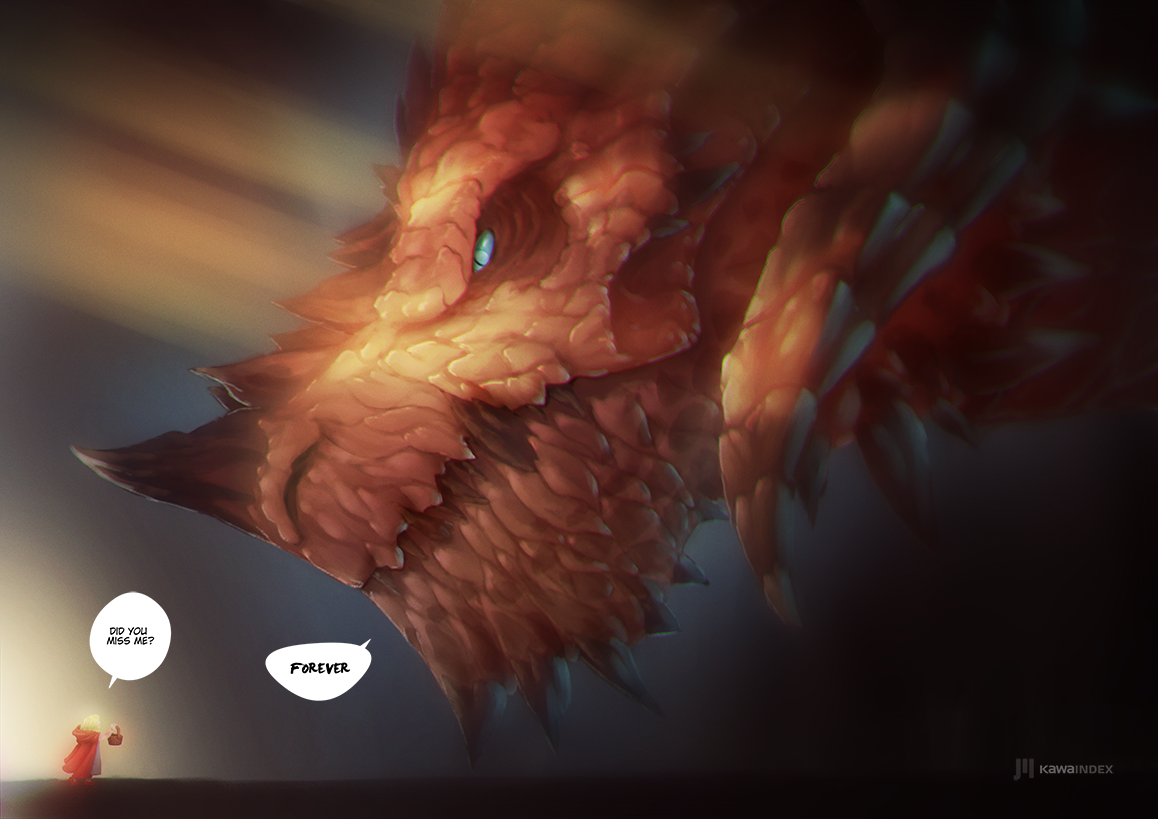
\includegraphics[width=\textwidth]{Figures/2X/Dragon/image.png}
            \caption{High Resolution}
        \end{subfigure}
        \vskip\baselineskip
        \begin{subfigure}[b]{0.475\textwidth}
            \centering
            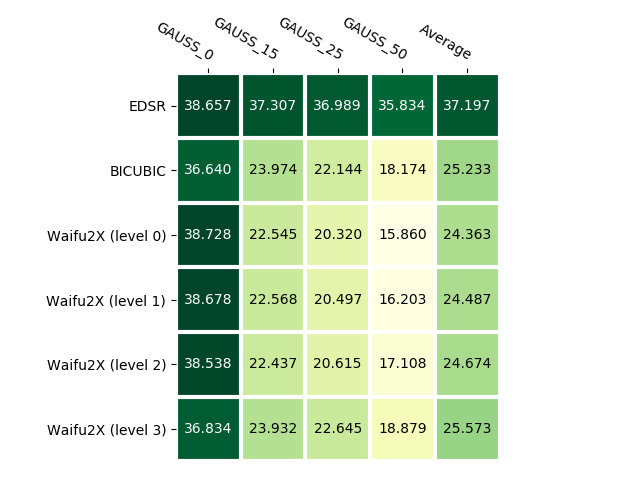
\includegraphics[width=\textwidth]{Figures/2X/Dragon/PSNR_GAUSS.png}
            \caption{PSNR results with gaussian noise}
        \end{subfigure}
        \hfill
        \begin{subfigure}[b]{0.475\textwidth}  
            \centering 
            \includegraphics[width=\textwidth]{Figures/2X/Dragon/PSNR_JPEG.png}
            \caption{PSNR results with JPEG noise}
        \end{subfigure}
        \vskip\baselineskip
        \begin{subfigure}[b]{0.475\textwidth}   
            \centering 
            \includegraphics[width=\textwidth]{Figures/2X/Dragon/SSIM_GAUSS.png}
            \caption{SSIM results with gaussian noise}
        \end{subfigure}
        \quad
        \begin{subfigure}[b]{0.475\textwidth}   
            \centering 
            \includegraphics[width=\textwidth]{Figures/2X/Dragon/SSIM_JPEG.png}
            \caption{SSIM results with JPEG noise}
        \end{subfigure}
        \caption{PSNR and SSIM results on the shown image}
    \end{figure*}
\chapter{Conclusion} % Main chapter title

\label{Chapter6}

My model achieves performance comparable to the best waifu2x model match for a given noise level for JPEG tasks, while dominating in gaussian denoising, I suspect the reason why it doesn't consistently outperform it in JPEG denoising (apart from the average score) is that the patch size is overly small (32 x 32), I used the L2 metric as a "safe" option since I was adding new functionality to the network apart from just uscaling, despite L1 having empirically better results (\cite{EDSR}) and the lack of Batch Normalization layers, which are proven to degrade performance slightly (\cite{DnCNN}), however the fact that my model performs substantially better when the picture has a lot of fine detail \ref{Cyberpunk_fig} suggest that there might actually be an overfitting issue, after all EDSR is a highly complex model, and artwork is generally not as complex as photographs.

\section{Future work}

I have found a small handful of images with compression artifacts that differ from JPEG compression, I will try to find the optimizer that generated those artifacts and include it in the training data, as well as other downsampling methods to fix aliasing or other issues that might occur on low resolution images.

%----------------------------------------------------------------------------------------
%	ABBREVIATIONS
%----------------------------------------------------------------------------------------

\begin{abbreviations}{ll} % Include a list of abbreviations (a table of two columns)

\textbf{CNN} & \textbf{C}onvolutional \textbf{N}eural \textbf{N}etwork\\
\textbf{GAN} & \textbf{G}enerative \textbf{A}dversarial \textbf{N}etwork\\
\textbf{GUI} & \textbf{G}raphical \textbf{U}ser \textbf{I}nterface \\
\textbf{JSON} & \textbf{J}ava \textbf{S}cript \textbf{O}bject \textbf{N}otation\\
\textbf{SR} & \textbf{S}uper \textbf{R}esolution\\
\textbf{HR} & \textbf{H}igh \textbf{R}esolution\\
\textbf{LR} & \textbf{L}ow \textbf{R}esolution\\
\textbf{SISR} & \textbf{S}ingle \textbf{I}mage \textbf{S}uper \textbf{R}esolution\\
\textbf{PSNR} & \textbf{P}eak \textbf{S}ignal to \textbf{N}oise \textbf{R}atio \\ 
\textbf{SSIM} & \textbf{S}tructural \textbf{SIM}ilarity Index\\

\end{abbreviations}

%----------------------------------------------------------------------------------------
%	ACKNOWLEDGEMENTS
%----------------------------------------------------------------------------------------

\begin{acknowledgements}
\addchaptertocentry{\acknowledgementname} % Add the acknowledgements to the table of contents
I thank my advisor for pointing me in the right direction with this project when he talked to me about the NITRE challenge and gave me the EDSR and CinCGAN papers to read, as a researcher in the field of Computer Vision he would know about the latest developments in Super-Resolution much better than a master degree student searching on Google Scholar.

\hfill

I also want to thank my colleague Jordan that left the program after the first semester for making that trial by fire bearable enough for me to get this far.

\end{acknowledgements}

%----------------------------------------------------------------------------------------
%	THESIS CONTENT - APPENDICES
%----------------------------------------------------------------------------------------

\appendix % Cue to tell LaTeX that the following "chapters" are Appendices

% Include the appendices of the thesis as separate files from the Appendices folder
% Uncomment the lines as you write the Appendices

% Appendix A

\chapter{Results for 3X scale} % Main appendix title

\label{AppendixA} % For referencing this appendix elsewhere, use \ref{AppendixA}

    \begin{figure*}
        \centering
        \begin{subfigure}[b]{0.75\textwidth}
            \centering
            \includegraphics[width=\textwidth]{Figures/2X/Cyberpunk/be15968553390b112e723e8773910e11.png}
            \caption{High Resolution}
        \end{subfigure}
        \vskip\baselineskip
        \begin{subfigure}[b]{0.475\textwidth}
            \centering
            \includegraphics[width=\textwidth]{Figures/3X/Cyberpunk/PSNR_GAUSS.png}
            \caption{PSNR results with gaussian noise}
        \end{subfigure}
        \hfill
        \begin{subfigure}[b]{0.475\textwidth}  
            \centering 
            \includegraphics[width=\textwidth]{Figures/3X/Cyberpunk/PSNR_JPEG.png}
            \caption{PSNR results with JPEG noise}
        \end{subfigure}
        \vskip\baselineskip
        \begin{subfigure}[b]{0.475\textwidth}   
            \centering 
            \includegraphics[width=\textwidth]{Figures/3X/Cyberpunk/SSIM_GAUSS.png}
            \caption{SSIM results with gaussian noise}
        \end{subfigure}
        \quad
        \begin{subfigure}[b]{0.475\textwidth}   
            \centering 
            \includegraphics[width=\textwidth]{Figures/3X/Cyberpunk/SSIM_JPEG.png}
            \caption{SSIM results with JPEG noise}
        \end{subfigure}
        \caption{PSNR and SSIM results on the shown image}
    \end{figure*}
    
    \begin{figure*}
        \centering
        \begin{subfigure}[b]{0.75\textwidth}
            \centering
            \includegraphics[width=\textwidth]{Figures/2X/Tiger/image.png}
            \caption{High Resolution}
        \end{subfigure}
        \vskip\baselineskip
        \begin{subfigure}[b]{0.475\textwidth}
            \centering
            \includegraphics[width=\textwidth]{Figures/3X/Tiger/PSNR_GAUSS.png}
            \caption{PSNR results with gaussian noise}
        \end{subfigure}
        \hfill
        \begin{subfigure}[b]{0.475\textwidth}  
            \centering 
            \includegraphics[width=\textwidth]{Figures/3X/Tiger/PSNR_JPEG.png}
            \caption{PSNR results with JPEG noise}
        \end{subfigure}
        \vskip\baselineskip
        \begin{subfigure}[b]{0.475\textwidth}   
            \centering 
            \includegraphics[width=\textwidth]{Figures/3X/Tiger/SSIM_GAUSS.png}
            \caption{SSIM results with gaussian noise}
        \end{subfigure}
        \quad
        \begin{subfigure}[b]{0.475\textwidth}   
            \centering 
            \includegraphics[width=\textwidth]{Figures/3X/Tiger/SSIM_JPEG.png}
            \caption{SSIM results with JPEG noise}
        \end{subfigure}
        \caption{PSNR and SSIM results on the shown image}
    \end{figure*}
    
        \begin{figure*}
        \centering
        \begin{subfigure}[b]{0.75\textwidth}
            \centering
            \includegraphics[width=\textwidth]{Figures/2X/Bear/image.png}
            \caption{High Resolution}
        \end{subfigure}
        \vskip\baselineskip
        \begin{subfigure}[b]{0.475\textwidth}
            \centering
            \includegraphics[width=\textwidth]{Figures/3X/Bear/PSNR_GAUSS.png}
            \caption{PSNR results with gaussian noise}
        \end{subfigure}
        \hfill
        \begin{subfigure}[b]{0.475\textwidth}  
            \centering 
            \includegraphics[width=\textwidth]{Figures/3X/Bear/PSNR_JPEG.png}
            \caption{PSNR results with JPEG noise}
        \end{subfigure}
        \vskip\baselineskip
        \begin{subfigure}[b]{0.475\textwidth}   
            \centering 
            \includegraphics[width=\textwidth]{Figures/3X/Bear/SSIM_GAUSS.png}
            \caption{SSIM results with gaussian noise}
        \end{subfigure}
        \quad
        \begin{subfigure}[b]{0.475\textwidth}   
            \centering 
            \includegraphics[width=\textwidth]{Figures/3X/Bear/SSIM_JPEG.png}
            \caption{SSIM results with JPEG noise}
        \end{subfigure}
        \caption{PSNR and SSIM results on the shown image}
    \end{figure*}
    
        \begin{figure*}
        \centering
        \begin{subfigure}[b]{0.75\textwidth}
            \centering
            \includegraphics[width=\textwidth]{Figures/2X/Catch/image.png}
            \caption{High Resolution}
        \end{subfigure}
        \vskip\baselineskip
        \begin{subfigure}[b]{0.475\textwidth}
            \centering
            \includegraphics[width=\textwidth]{Figures/3X/Catch/PSNR_GAUSS.png}
            \caption{PSNR results with gaussian noise}
        \end{subfigure}
        \hfill
        \begin{subfigure}[b]{0.475\textwidth}  
            \centering 
            \includegraphics[width=\textwidth]{Figures/3X/Catch/PSNR_JPEG.png}
            \caption{PSNR results with JPEG noise}
        \end{subfigure}
        \vskip\baselineskip
        \begin{subfigure}[b]{0.475\textwidth}   
            \centering 
            \includegraphics[width=\textwidth]{Figures/3X/Catch/SSIM_GAUSS.png}
            \caption{SSIM results with gaussian noise}
        \end{subfigure}
        \quad
        \begin{subfigure}[b]{0.475\textwidth}   
            \centering 
            \includegraphics[width=\textwidth]{Figures/3X/Catch/SSIM_JPEG.png}
            \caption{SSIM results with JPEG noise}
        \end{subfigure}
        \caption{PSNR and SSIM results on the shown image}
    \end{figure*}
    
            \begin{figure*}
        \centering
        \begin{subfigure}[b]{0.75\textwidth}
            \centering
            \includegraphics[width=\textwidth]{Figures/2X/Coffee/image.png}
            \caption{High Resolution}
        \end{subfigure}
        \vskip\baselineskip
        \begin{subfigure}[b]{0.475\textwidth}
            \centering
            \includegraphics[width=\textwidth]{Figures/3X/Coffee/PSNR_GAUSS.png}
            \caption{PSNR results with gaussian noise}
        \end{subfigure}
        \hfill
        \begin{subfigure}[b]{0.475\textwidth}  
            \centering 
            \includegraphics[width=\textwidth]{Figures/3X/Coffee/PSNR_JPEG.png}
            \caption{PSNR results with JPEG noise}
        \end{subfigure}
        \vskip\baselineskip
        \begin{subfigure}[b]{0.475\textwidth}   
            \centering 
            \includegraphics[width=\textwidth]{Figures/3X/Coffee/SSIM_GAUSS.png}
            \caption{SSIM results with gaussian noise}
        \end{subfigure}
        \quad
        \begin{subfigure}[b]{0.475\textwidth}   
            \centering 
            \includegraphics[width=\textwidth]{Figures/3X/Coffee/SSIM_JPEG.png}
            \caption{SSIM results with JPEG noise}
        \end{subfigure}
        \caption{PSNR and SSIM results on the shown image}
    \end{figure*}
    
            \begin{figure*}
        \centering
        \begin{subfigure}[b]{0.75\textwidth}
            \centering
            \includegraphics[width=\textwidth]{Figures/2X/Crow/image.png}
            \caption{High Resolution}
        \end{subfigure}
        \vskip\baselineskip
        \begin{subfigure}[b]{0.475\textwidth}
            \centering
            \includegraphics[width=\textwidth]{Figures/3X/Crow/PSNR_GAUSS.png}
            \caption{PSNR results with gaussian noise}
        \end{subfigure}
        \hfill
        \begin{subfigure}[b]{0.475\textwidth}  
            \centering 
            \includegraphics[width=\textwidth]{Figures/3X/Crow/PSNR_JPEG.png}
            \caption{PSNR results with JPEG noise}
        \end{subfigure}
        \vskip\baselineskip
        \begin{subfigure}[b]{0.475\textwidth}   
            \centering 
            \includegraphics[width=\textwidth]{Figures/3X/Crow/SSIM_GAUSS.png}
            \caption{SSIM results with gaussian noise}
        \end{subfigure}
        \quad
        \begin{subfigure}[b]{0.475\textwidth}   
            \centering 
            \includegraphics[width=\textwidth]{Figures/3X/Crow/SSIM_JPEG.png}
            \caption{SSIM results with JPEG noise}
        \end{subfigure}
        \caption{PSNR and SSIM results on the shown image}
    \end{figure*}
    
            \begin{figure*}
        \centering
        \begin{subfigure}[b]{0.75\textwidth}
            \centering
            \includegraphics[width=\textwidth]{Figures/2X/Dragon/image.png}
            \caption{High Resolution}
        \end{subfigure}
        \vskip\baselineskip
        \begin{subfigure}[b]{0.475\textwidth}
            \centering
            \includegraphics[width=\textwidth]{Figures/3X/Dragon/PSNR_GAUSS.png}
            \caption{PSNR results with gaussian noise}
        \end{subfigure}
        \hfill
        \begin{subfigure}[b]{0.475\textwidth}  
            \centering 
            \includegraphics[width=\textwidth]{Figures/3X/Dragon/PSNR_JPEG.png}
            \caption{PSNR results with JPEG noise}
        \end{subfigure}
        \vskip\baselineskip
        \begin{subfigure}[b]{0.475\textwidth}   
            \centering 
            \includegraphics[width=\textwidth]{Figures/3X/Dragon/SSIM_GAUSS.png}
            \caption{SSIM results with gaussian noise}
        \end{subfigure}
        \quad
        \begin{subfigure}[b]{0.475\textwidth}   
            \centering 
            \includegraphics[width=\textwidth]{Figures/3X/Dragon/SSIM_JPEG.png}
            \caption{SSIM results with JPEG noise}
        \end{subfigure}
        \caption{PSNR and SSIM results on the shown image}
    \end{figure*}
% Appendix B

\chapter{Results for 4X scale} % Main appendix title

\label{AppendixB} % For referencing this appendix elsewhere, use \ref{AppendixB}

    \begin{figure*}
        \centering
        \begin{subfigure}[b]{0.75\textwidth}
            \centering
            \includegraphics[width=\textwidth]{Figures/2X/Cyberpunk/be15968553390b112e723e8773910e11.png}
            \caption{High Resolution}
        \end{subfigure}
        \vskip\baselineskip
        \begin{subfigure}[b]{0.475\textwidth}
            \centering
            \includegraphics[width=\textwidth]{Figures/4X/Cyberpunk/PSNR_GAUSS.png}
            \caption{PSNR results with gaussian noise}
        \end{subfigure}
        \hfill
        \begin{subfigure}[b]{0.475\textwidth}  
            \centering 
            \includegraphics[width=\textwidth]{Figures/4X/Cyberpunk/PSNR_JPEG.png}
            \caption{PSNR results with JPEG noise}
        \end{subfigure}
        \vskip\baselineskip
        \begin{subfigure}[b]{0.475\textwidth}   
            \centering 
            \includegraphics[width=\textwidth]{Figures/4X/Cyberpunk/SSIM_GAUSS.png}
            \caption{SSIM results with gaussian noise}
        \end{subfigure}
        \quad
        \begin{subfigure}[b]{0.475\textwidth}   
            \centering 
            \includegraphics[width=\textwidth]{Figures/4X/Cyberpunk/SSIM_JPEG.png}
            \caption{SSIM results with JPEG noise}
        \end{subfigure}
        \caption{PSNR and SSIM results on the shown image}
    \end{figure*}
    
    \begin{figure*}
        \centering
        \begin{subfigure}[b]{0.75\textwidth}
            \centering
            \includegraphics[width=\textwidth]{Figures/2X/Tiger/image.png}
            \caption{High Resolution}
        \end{subfigure}
        \vskip\baselineskip
        \begin{subfigure}[b]{0.475\textwidth}
            \centering
            \includegraphics[width=\textwidth]{Figures/4X/Tiger/PSNR_GAUSS.png}
            \caption{PSNR results with gaussian noise}
        \end{subfigure}
        \hfill
        \begin{subfigure}[b]{0.475\textwidth}  
            \centering 
            \includegraphics[width=\textwidth]{Figures/4X/Tiger/PSNR_JPEG.png}
            \caption{PSNR results with JPEG noise}
        \end{subfigure}
        \vskip\baselineskip
        \begin{subfigure}[b]{0.475\textwidth}   
            \centering 
            \includegraphics[width=\textwidth]{Figures/4X/Tiger/SSIM_GAUSS.png}
            \caption{SSIM results with gaussian noise}
        \end{subfigure}
        \quad
        \begin{subfigure}[b]{0.475\textwidth}   
            \centering 
            \includegraphics[width=\textwidth]{Figures/4X/Tiger/SSIM_JPEG.png}
            \caption{SSIM results with JPEG noise}
        \end{subfigure}
        \caption{PSNR and SSIM results on the shown image}
    \end{figure*}
    
        \begin{figure*}
        \centering
        \begin{subfigure}[b]{0.75\textwidth}
            \centering
            \includegraphics[width=\textwidth]{Figures/2X/Bear/image.png}
            \caption{High Resolution}
        \end{subfigure}
        \vskip\baselineskip
        \begin{subfigure}[b]{0.475\textwidth}
            \centering
            \includegraphics[width=\textwidth]{Figures/4X/Bear/PSNR_GAUSS.png}
            \caption{PSNR results with gaussian noise}
        \end{subfigure}
        \hfill
        \begin{subfigure}[b]{0.475\textwidth}  
            \centering 
            \includegraphics[width=\textwidth]{Figures/4X/Bear/PSNR_JPEG.png}
            \caption{PSNR results with JPEG noise}
        \end{subfigure}
        \vskip\baselineskip
        \begin{subfigure}[b]{0.475\textwidth}   
            \centering 
            \includegraphics[width=\textwidth]{Figures/4X/Bear/SSIM_GAUSS.png}
            \caption{SSIM results with gaussian noise}
        \end{subfigure}
        \quad
        \begin{subfigure}[b]{0.475\textwidth}   
            \centering 
            \includegraphics[width=\textwidth]{Figures/4X/Bear/SSIM_JPEG.png}
            \caption{SSIM results with JPEG noise}
        \end{subfigure}
        \caption{PSNR and SSIM results on the shown image}
    \end{figure*}
    
        \begin{figure*}
        \centering
        \begin{subfigure}[b]{0.75\textwidth}
            \centering
            \includegraphics[width=\textwidth]{Figures/2X/Catch/image.png}
            \caption{High Resolution}
        \end{subfigure}
        \vskip\baselineskip
        \begin{subfigure}[b]{0.475\textwidth}
            \centering
            \includegraphics[width=\textwidth]{Figures/4X/Catch/PSNR_GAUSS.png}
            \caption{PSNR results with gaussian noise}
        \end{subfigure}
        \hfill
        \begin{subfigure}[b]{0.475\textwidth}  
            \centering 
            \includegraphics[width=\textwidth]{Figures/4X/Catch/PSNR_JPEG.png}
            \caption{PSNR results with JPEG noise}
        \end{subfigure}
        \vskip\baselineskip
        \begin{subfigure}[b]{0.475\textwidth}   
            \centering 
            \includegraphics[width=\textwidth]{Figures/4X/Catch/SSIM_GAUSS.png}
            \caption{SSIM results with gaussian noise}
        \end{subfigure}
        \quad
        \begin{subfigure}[b]{0.475\textwidth}   
            \centering 
            \includegraphics[width=\textwidth]{Figures/4X/Catch/SSIM_JPEG.png}
            \caption{SSIM results with JPEG noise}
        \end{subfigure}
        \caption{PSNR and SSIM results on the shown image}
    \end{figure*}
    
            \begin{figure*}
        \centering
        \begin{subfigure}[b]{0.75\textwidth}
            \centering
            \includegraphics[width=\textwidth]{Figures/2X/Coffee/image.png}
            \caption{High Resolution}
        \end{subfigure}
        \vskip\baselineskip
        \begin{subfigure}[b]{0.475\textwidth}
            \centering
            \includegraphics[width=\textwidth]{Figures/4X/Coffee/PSNR_GAUSS.png}
            \caption{PSNR results with gaussian noise}
        \end{subfigure}
        \hfill
        \begin{subfigure}[b]{0.475\textwidth}  
            \centering 
            \includegraphics[width=\textwidth]{Figures/4X/Coffee/PSNR_JPEG.png}
            \caption{PSNR results with JPEG noise}
        \end{subfigure}
        \vskip\baselineskip
        \begin{subfigure}[b]{0.475\textwidth}   
            \centering 
            \includegraphics[width=\textwidth]{Figures/4X/Coffee/SSIM_GAUSS.png}
            \caption{SSIM results with gaussian noise}
        \end{subfigure}
        \quad
        \begin{subfigure}[b]{0.475\textwidth}   
            \centering 
            \includegraphics[width=\textwidth]{Figures/4X/Coffee/SSIM_JPEG.png}
            \caption{SSIM results with JPEG noise}
        \end{subfigure}
        \caption{PSNR and SSIM results on the shown image}
    \end{figure*}
    
            \begin{figure*}
        \centering
        \begin{subfigure}[b]{0.75\textwidth}
            \centering
            \includegraphics[width=\textwidth]{Figures/2X/Crow/image.png}
            \caption{High Resolution}
        \end{subfigure}
        \vskip\baselineskip
        \begin{subfigure}[b]{0.475\textwidth}
            \centering
            \includegraphics[width=\textwidth]{Figures/4X/Crow/PSNR_GAUSS.png}
            \caption{PSNR results with gaussian noise}
        \end{subfigure}
        \hfill
        \begin{subfigure}[b]{0.475\textwidth}  
            \centering 
            \includegraphics[width=\textwidth]{Figures/4X/Crow/PSNR_JPEG.png}
            \caption{PSNR results with JPEG noise}
        \end{subfigure}
        \vskip\baselineskip
        \begin{subfigure}[b]{0.475\textwidth}   
            \centering 
            \includegraphics[width=\textwidth]{Figures/4X/Crow/SSIM_GAUSS.png}
            \caption{SSIM results with gaussian noise}
        \end{subfigure}
        \quad
        \begin{subfigure}[b]{0.475\textwidth}   
            \centering 
            \includegraphics[width=\textwidth]{Figures/4X/Crow/SSIM_JPEG.png}
            \caption{SSIM results with JPEG noise}
        \end{subfigure}
        \caption{PSNR and SSIM results on the shown image}
    \end{figure*}
    
            \begin{figure*}
        \centering
        \begin{subfigure}[b]{0.75\textwidth}
            \centering
            \includegraphics[width=\textwidth]{Figures/2X/Dragon/image.png}
            \caption{High Resolution}
        \end{subfigure}
        \vskip\baselineskip
        \begin{subfigure}[b]{0.475\textwidth}
            \centering
            \includegraphics[width=\textwidth]{Figures/4X/Dragon/PSNR_GAUSS.png}
            \caption{PSNR results with gaussian noise}
        \end{subfigure}
        \hfill
        \begin{subfigure}[b]{0.475\textwidth}  
            \centering 
            \includegraphics[width=\textwidth]{Figures/4X/Dragon/PSNR_JPEG.png}
            \caption{PSNR results with JPEG noise}
        \end{subfigure}
        \vskip\baselineskip
        \begin{subfigure}[b]{0.475\textwidth}   
            \centering 
            \includegraphics[width=\textwidth]{Figures/4X/Dragon/SSIM_GAUSS.png}
            \caption{SSIM results with gaussian noise}
        \end{subfigure}
        \quad
        \begin{subfigure}[b]{0.475\textwidth}   
            \centering 
            \includegraphics[width=\textwidth]{Figures/4X/Dragon/SSIM_JPEG.png}
            \caption{SSIM results with JPEG noise}
        \end{subfigure}
        \caption{PSNR and SSIM results on the shown image}
    \end{figure*}

%----------------------------------------------------------------------------------------
%	BIBLIOGRAPHY
%----------------------------------------------------------------------------------------

\printbibliography[heading=bibintoc]

%----------------------------------------------------------------------------------------

\end{document}  
